\part{排名理论}

%\ornamento
\chapter{社会选择理论}
人类行为是由一系列选择(choice)和决策(decision making)构成,理解人类行为的一切思想都以研究选择为基础,如古希腊先哲苏格拉底(Socrates)和亚里斯多德
(Aristotle)认为愿望和信仰是人类做出选择的前提。19世纪,人们开始构建人类选择的量化模型,比如实验心理学的奠基人恩斯特·海因里希·韦伯Ernst Heinrich Weber 通过建立心理活动和可度量物理行为间的关联,提出著名的\textbf{韦伯定律},成为心理学量化分析人类心理活动(包括选择)的基石。承其衣钵的学生古斯塔夫·费希纳Gustav Theodor Fechner扩展韦伯定律,创立出更为精确的度量系统,称作\textbf{费希纳定律}。20世纪初,法国路易斯· 列昂· 瑟斯顿Louis Leon Thurstone
\footnote{路易斯· 列昂· 瑟斯顿Louis Leon Thurstone(1887-1955),美国心理学家,美国心理测量学会的创立者之一,并任第一届心理测量学会主席,在测量理论、社会评价等理论应用方面均作出巨大贡献。1933年当选为美国心理学会主席,1938年当选为国家科学院院士。}
基于韦伯--费希纳定律发展出比较性评价(comparative judgment)系统~\cite{thurstone1927method},基于成对比较的瑟斯顿模型由此诞生。

社会选择(social choice),也称“集体决策”(collective decision)是将社会成员的个人意愿或偏好汇集成群体意愿或偏好的过程,属于典型的群体决策问题。选举制度是社会选择的一个制度性体现,为民主国家反映民意的一个主要机制。为了体现少数服从多数的民主理念,人们提出\textbf{多数代表制}(majoritarian representation)或\textbf{多数制}(plurality voting),认定得票最多的候选人胜出。为了确保反映社会多元化的意见,1846年瑞士学者Victor Considerant提出
\textbf{比例代表制}(proportional representation),根据政党或参选组别得票比例分配议席。由于不同选区人口或经济地位的差异,人们根据每个选区所代表的议席数目,将选举方法分成\textbf{单一选区制}(single-member district)或“小选区制”(small constituency system)、\textbf{复数选区制}(multi-member district)或“大选区制”(large-size district)。单一选区制每个选区只有一个议席,而复数选区制每个选区对应多个议席。多数制在单一选区制下也称作\textbf{简单多数制}(first-past-the-post, single choice voting, simple plurality, simple majority)或\textbf{相对多数制}(relative majority)
\footnote{多数制别称相对多数制,与之对应的是绝对多数制(absolute majority):候选人得票数只有超过其他候选人得票数之和才算胜出。};在复数选区制下称作
\textbf{胜者全拿}(winer-takes-all)。如果根据选举规则无法选出一个合适的候选人,可能是平局,也可能是不满足一定的规则,为避免出现此类状况,人们提出
\textbf{决胜选举}(run-off)进行多轮投票直至有人胜出。

我们将在后续章节介绍社会选择的相关概念、公理性推导、社会选择方法与投票准则、评价社会选择的标准、各种社会选择方法的关联以及几个著名的社会选择悖论,最后介绍社会选择理论最新进展\textbf{计算社会选择}(Computational Social Choice,CSC),以及社会选择理论在推荐系统评分预测、网络排名聚合、体育竞技排名等领域的应用研究。

\section{符号定义}
社会选择通常依赖于可排列对象的排列变换(permutation)
\footnote{英文单词Permutation存在两个中文字面翻译:\textbf{排列}或\textbf{置换}。本文对两种翻译不作具体区分,主要使用第一种翻译意思。当permutation作为一个变换算子出现时,我们称其\textbf{排列变换};当permutation作为一个有序列表出现时,我们称其\textbf{排名列表}。读者如果对排列和置换之间的差异感兴趣,可参考潘庆年教授的一篇注解\cite{pan1998note}。},为此我们对相关概念给出统一的数学定义。假设$\mathcal A = \{x,y,z,\ldots\}$是可排序
\footnote{可排序依赖于空间上定义的二元全序关系,我们将在后文给出严格定义。}
的对象集,如决策时的备择选项(alternatives)、选举投票时的候选人集合(candidates)、在线购物评分时的商品列表(items)等,并且$|\mathcal A|=n$,$\mathcal A$上的一个\textbf{排列}(ranking \textit{or} ballot)定义为从$\mathcal A$ 到$\{1,2,\ldots,n\}$上的一个双射:
\begin{equation}\label{eq:permutation}
    \pi: \mathcal A \mapsto \{1,2,\ldots,n\},
\end{equation}
并使用$\pi(i)$表示$\mathcal A$中第$i$个对象在排列变换$\pi$作用下的排名,$\pi^{-1}(i)$表示在$\pi$作用下排在第$i$位的原始对象。通常,我们也使用$\pi$和$\pi^{-1}$ 分别表示由$\mathcal A$中所有对象的排名向量、有序排列的对象向量。对象集$\mathcal A$可以产生$n!$种可能的全排列组合,可以构成一个非交换群,记为$\Pi[\mathcal A]$或$\Pi[n]$。 如果我们选择一部分对象,比如$\{\pi^{-1}(1), \pi^{-1}(2), \ldots, \pi^{-1}(K)\}$,从群$\Pi[n]$中筛选出所有第$i$ 位对应$\pi^{-1}(i)$ 的排列,$1\le i\le K \le n$,构成$\Pi[n]$ 的一个子群,记作$\Pi[n,K, \pi]$:
\begin{equation}\label{eq:subgroup}
    \Pi[n,K,\pi] = \big\{\sigma\in \Pi(n)|\sigma^{-1}(i) = \pi^{-1}(i), 1\le i \le K\big\}.
\end{equation}
假设存在一组决策者$\mathcal M=\{X,Y,Z,\ldots\}$,比如投票选举时的选民(voters)、电影评价时的影评人(raters)等,并且$|\mathcal M|=m$,每个决策者都有一个$\mathcal A$上的个人偏好排名(individual preferential ranking),从而构成一个\textbf{社会偏好集}(social preference profile)
\begin{equation}\label{eq:preferenceprofile}
    \Pi[\mathcal A,\mathcal M]=\Pi[n,m]=\{\pi_i\}_{i=1}^m\in  \Omega[n,m],
\end{equation}
其中$\pi_i\in \Pi[n]$表示$\mathcal M$上第$i$个决策者对$\mathcal A$ 做出的一个线性排序,$\Omega[n,m]$是$\mathcal M$在$\mathcal A$上所有可能的偏好集,且有$|\Omega[n,m]|=(n!)^m$。在不产生混淆的情况下,我们简记作$\Pi\triangleq \Pi[n,m]$。 如果存在一个社会选择函数$\mathcal F: \Pi[n,m]\mapsto \Pi[n]$,能够基于$\Pi[n,m]$ 给出$\mathcal A$ 的一个全局性的评价,则全局线性排序记作$\pi_{\mathcal F}\in \Pi[n]$,也成社会偏好排名(social preferential ranking)。 对于任意一个$\mathcal A$上的线性序$\pi$,都对应一个特殊的决策方。给定任意两个对象$x,y\in \mathcal A$,我们用$x\succ_\pi y$ 表示$x$ 在$\pi$中的排名高于$y$,或者$\pi$偏好$x$甚于$y$。为了强调决策方,比如决策者$Z$偏好$x$甚于$y$,则记作$x\succ_Z y$。如果$\mathcal F$ 偏好$x$甚于$y$,则记作$x\succ_{\Pi[n,m]}^{\mathcal F} y$,或简记作$x\succ_\Pi^{\mathcal F} y$。如果存在一个社会选择函数$\mathcal F:\Pi[n,m]\mapsto \mathcal A$,则它能够基于$\Pi[n,m]$选择$\mathcal A$上的一个成员,并称其为社会选择(social choice)。我们根据大量决策者的偏好信息,从而确定出$\mathcal A$中的一个成员或者全体社会对$\mathcal A$的整体偏好。如果细分两种情形,则前者对应一个社会选择函数$\mathcal F: \Pi[n,m]\mapsto \Pi[n]$;后者对应一个社会福利函数$\mathcal F: \Pi[n,m]\mapsto \mathcal A$。
\begin{example}\label{eg:gallup-2016}
    2014年7月7日至10日,盖洛普(Gallup)对民主党五位2016年总统选举候选人Hillary Clinton、Elizabeth Warren、Andrew Cuomo、Martin O'Malley、Joe Biden组织了一次民意调查
    \footnote{Gallup: \href{http://www.gallup.com/poll/173402/clinton-best-known-best-liked-potential-2016-candidate.aspx}{\textit{Clinton Is Best Known, Best Liked Potential 2016 Candidate}}, 2015-09-14},
    统计公众对几位候选人的了解情况,具体统计数据见下表:
    \begin{table}[htbp]
        \centering
        \begin{tabular}{lcccc}
          \hline
          Candidate & Familiar (\%) & Favorable (\%) & Unfavorable (\%) & Net Favorable (\%)\\
          \hline
          Hillary Clinton & 91 & 55 & 36 & 19\\
          Elizabeth Warren & 38 & 21 & 17 & 4\\
          Andrew Cuomo & 51 & 27 & 24 & 3\\
          Martin O'Malley & 19 & 7 & 9 & -2\\
          Joe Biden & 80 & 38 & 42 & -4\\
          \hline
        \end{tabular}
        \caption{2014年7月7日至10日盖洛普民主党2016总统候选人民调数据}
        \label{tbl:gallup-2016}
    \end{table}
    表格中每一行代表一位候选人,第二列是公众认识候选人的比例,第三列是公众认同候选人的比例,第四列是公众不认同候选人的比例,最后一列则是公众认同候选人减去不认同的比例,属于净认同的比例。根据数据可知,五位总统候选人$\mathcal A=\big\{$Clinton,Warren,Cuomo,O'Malley,Biden$\big\}$中,美国前第一夫人、前国务卿Clinton是公众最为熟知、最受公众欢迎的民主党候选人。前副总统Biden虽为公众所知,认同他的民众却少于不认同他的人数。

    我们现在用一组连续的自然数$\{1,2,3,4,5\}$为他们编号,则1号对应Clinton,3号对应Cuomo。如果根据第二列的公众熟知比例为他们排名,则会产生一个新的排名列表$\pi_1=\langle 1, 4, 3, 5, 2\rangle$,那么$\pi_1^{-1}(4)=2$表示排名列表$\pi_1$中位列第4的对象是2号候选人Warren,$\pi_1(5)=2$表示5号候选人Biden 在列表$\pi_1$ 中排名第2 位。类似地,我们按照最后一列排列候选人名单,又会产生一个排名列表$\pi_4=\langle1, 2, 3, 4, 5\rangle$。
\end{example}

我们根据社会选择法的步骤及输出数据类型\cite{riker1982liberalism,farah2007outranking},将社会选择方法分成位置评分法、位置筛选法和概率模型法。位置评分准则赋予每个候选人一个对应分值,分值的产生可能源于整体排序(如波达计数\cite{borda1781m}、Footrule法\cite{marden1995analyzing}、中位数法
\cite{fagin2003efficient}、CPS模型\cite{qin2010new} 和矩阵分解方法\cite{gleich2011rank}),或者源于序对比较(如孔多塞法、凯梅尼─杨格方法和马尔科夫方法)。位置筛选法综合候选人的位置、多数投票得分等因素,逐步缩短偏好列表的长度,剔除不合格的候选人直至最优人选诞生,如单记可让渡投票制。概率模型法建立候选人排列的概率分布,包括瑟斯顿模型~\cite{thurstone1927method}、 布雷德利─特里模型~\cite{bradley1952rank}、 马洛斯模型~\cite{mallows1957non} 和普拉基特─卢斯模型~\cite{luce1959individual,plackett1975analysis}。我们在后续几个小节简要介绍几种代表性的社会选择方法,并基于1980年美国参议院议员选举为例解释各种方法。

\begin{example}\cite{taylor2008mathematics}
1980年美国纽约州参议院选举在保守派的Alphonse D'Amato、自由派的Elizabeth Holtzman与Jacob Javits之间展开,三名候选人的得票率如表\ref{tbl:1980ussenate}所示,22\%的选民对于三名候选人的个人偏好为$D\succ H\succ J$,4\%的选民存在个人偏好$J\succ D\succ H$,每名候选人使用其姓氏首字母表示。为简化表示,我们在后续章节使用本例数据时直接省略百分号。
\begin{table}[ht]
    \centering
    \begin{tabular}{c|c|c|c|c|c}
      \hline
      29\% & 23\% & 22\% & 15\% & 7\% & 4\%\\
      \hline
      H & D & D & H & J & J\\
      J & J & H & D & H & D\\
      D & H & J & J & D & H\\
      \hline
    \end{tabular}
    \caption{1980年美国纽约州参议院选举}
    \label{tbl:1980ussenate}
\end{table}
\end{example}\label{eg:1980usny}

\section{位置评分法}
位置评分法根据每个偏好列表对所有候选人评分,然后累加候选人在所有偏好集上评分得到总的分值,利用各候选人的综合评分可以选出优胜者或者建立所有候选人的综合排名。假设$V_\pi\in \mathbb R^n$表示$\mathcal A$在偏好列表$\pi$上的得分向量,则$\mathcal A$内所有候选人的综合得分向量
\begin{equation}
    V_\Pi=V_\Pi = \sum\limits_{\pi\in \Pi}V_\pi = \sum\limits_{\pi\in \Pi} \bigg(V_\pi^1,V_\pi^2, \ldots, V_\pi^n\bigg),
\end{equation}
其中$V_\pi^i$表示$\mathcal A$中第$i$个候选人在偏好列表$\pi$下的得分分值,$1\le i\le n$。

\subsection{多数投票法}
多数投票法是一种最常见的投票选择方法,也是英国大选采用的一种选举方法。它只利用所有偏好列表排名第一的数据确定出最终赢家。对于某个选民偏好列表$\pi$,根据候选人集合$\mathcal A$ 在偏好名单$\pi$上的名次,只有排名第一的候选人可以得到一个点数,其他位置上的候选人没有得分。对于例子\ref{eg:1980usny},多数投票法只考虑排名第一的候选人,各候选人的得分如下:
\[
    \text{$V_D$ = 23 + 22 = 45,$V_H$ = 29 + 15 = 44,$V_J$ = 7 + 4 = 11},
\]
候选人D'Amato以45比44险胜Holtzman,社会偏好为$D\succ H\succ J$。

\subsection{波达计数}
1770年,法国数学家、政治学家让─查尔斯·波达Jean-Charles de Borda\cite{borda1781m}设计出一种新的投票计数方法,称作\textbf{波达计数}(Borda Count),用于评选法国科学院院士。波达计数根据选民偏好名单中的排名给候选人一定的点数,一般地排名越高点数越高,如排名第一的候选人得到$n-1$个点,排名靠后依次逐渐减少一个点。后来,由于波拿巴·拿破仑的干预,弃用波达计数,并采纳拉普拉斯的意见,使用绝对多数准则评选科学院院士。根据波达计数法,例\ref{eg:1980usny}三名候选人得分
\[
    \begin{bmatrix}
        V_D\\
        V_H\\
        V_J\\
    \end{bmatrix} = 
    \begin{bmatrix}
      0 & 2 & 2 & 1 & 0 & 1\\
      2 & 0 & 1 & 2 & 1 & 0\\
      1 & 1 & 0 & 0 & 2 & 2\\
    \end{bmatrix}
    \times 
    \begin{bmatrix}
        \vspace{-0.3cm}
        \text{29}\\
        \vspace{-0.3cm}
        \text{23}\\
        \vspace{-0.3cm}
        \text{22}\\
        \vspace{-0.3cm}
        \text{15}\\
        \vspace{-0.3cm}
        \text{7}\\
        \vspace{-0.3cm}
        \text{4}\\
        \vspace{-0.3cm}
    \end{bmatrix} =
    \begin{bmatrix}
        \text{109}\\
        \text{115}\\
        \text{74}\\
    \end{bmatrix},
\]
可知候选人Holtzman胜出,社会偏好为$H\succ D\succ J$。

\subsection{计分投票法}
多数投票法与波达计数都是建立在排序投票系统之上,选民只是根据自己的偏好对候选人进行排列。实际上,如果选民能够对候选人进行顺次排序,我们可以给予其更多的自由,使用限定的离散分值给候选人打分,从而能够更有效地反映出选民的意愿。这种投票选举的方法称作\textbf{计分投票法}(range voting,rating summation,scoring),在网络空间有广泛应用,比如网民对电影、图书、商品的1--5级评分。计分投票法根据每个候选人所有评分均值、中值(majority judgment)或加和,评分最高者胜出。如果离散分值只有两个$\{0,1\}$或者$\{$同意,反对$\}$,则称计分投票法为\textbf{同意投票法}(approve voting)。我们可以从计分投票中构建每个选民的偏好排名,允许一对一的对决,满足各种良好的性质,如传递性、一致性等。可以如果存在策略性投票行为,由于每张选票每个候选人的可能分值是一个区间范围,即便是离散数字,也比排名列表形式的选票更难操纵。

\subsection{孔多塞方法}
1785年,法国启蒙思想家马奎斯·孔多塞Marquis de Condorcet\cite{condorcet1785essai}在研究民主决策时,提出一种序对型选举投票方法,称为\textbf{孔多塞方法}。孔多塞方法根据选民的偏好集合$\Pi$,统计所有可能的偏好序对,根据多数准则选出得票最多的赢家。如果$\Pi$存在一个候选人(比如$x$),在和其他每个候选人一对一对决(round-robin \textit{or} one-on-one \textit{or} head-to-head)
\footnote{体育运动竞技比赛,如网球、足球、国际象棋、桥牌、拳击运动,经常要运动员或团队之间进行多轮形式的循环赛(\textit{round-robin tournament}),表示所有参赛选手彼此进行多次两两对决。17世纪初,\textit{round-robin}衍生出新的涵义,表示“圆形签名请愿书”。在签署控诉书、请愿书等多人署名文件时,顺着一个圆圈署名,籍此让人分不出署名的先后顺序,以保护领头人免于遭受报复。}
时,都能获得多数选票,即有
\begin{equation}
    \forall y \in \mathcal A,~~\big|\{\pi\in \Pi: x\succ_\pi y\}\big| > \big|\{\pi\in \Pi: y\succ_\pi x\}\big|\text{,或} x\succ_\Pi^\mathcal{F'} y\text{,}
\end{equation}
则称其\textbf{孔多塞赢家}(Condorcet winner),其中$\mathcal{F'}$是多数投票法。根据孔多塞方法,例子\ref{eg:1980usny}中三个候选人的一对一对决统计结果如表\ref{tbl:condorcetwinner} 所示,候选人Holtzman是一个孔多塞赢家,并且社会偏好为$H\succ D\succ J$。
\begin{table}[ht]
    \centering
    \begin{tabular}{c|c|c}
      \hline
      偏好 & 得票 & 偏好\\
      \hline
      $H\succ D$ & 51 $>$ 49 & $D\succ H$\\
      $H\succ J$ & 66 $>$ 34 & $J\succ H$\\
      $D\succ J$ & 60 $>$ 40 & $J\succ D$\\
      \hline
    \end{tabular}
    \caption{孔多塞赢家}
    \label{tbl:condorcetwinner}
\end{table}
如果一个候选人是$\Pi[n]$上的孔多塞赢家,则它在一对一对决中从未被其他候选人击败,即是说其他每个候选人至少被此孔多塞赢家所击败一次,他们不可能是孔多塞赢家。由此可知,孔多塞赢家只要存在必然唯一,但它并非总是存在。
\begin{example}
假设某次社会投票选举只有三个候选人$\{x,y,z\}$参选,他们的偏好集如表\ref{tbl:condorcetsparadox}所示。根据孔多塞方法,统计每个候选人一对一对决结果,比如有20个选民存在偏好$x\succ y$,只有10个选民有偏好$y\succ x$,前者得两票胜出,则$x\succ y$;类似可知$y\succ z$与$z\succ x$。孔多塞方法在此社会偏好集上产生一个偏好回路(preferential cycle)$x\succ y\succ z\succ x$,存在一个内在矛盾:社会偏好$x$甚于$y$,偏好$y$甚于$z$,但又偏好$z$甚于$x$,孔多塞赢家并不存在,出现孔多塞悖论(Condorcet's paradox)。
\begin{table}[ht]
    \centering
    \begin{minipage}[t]{0.3\linewidth}
    \centering
    \begin{tabular}{c|c}
      \hline
      票数 & 偏好列表\\
      \hline
      10 & $x\succ y \succ z$\\
      10 & $y\succ z \succ x$\\
      10 & $z\succ x \succ y$\\
      \hline
    \end{tabular}
    \end{minipage}
    \begin{minipage}[t]{0.3\linewidth}
    \centering
    \begin{tabular}{c|c|c}
      \hline
      偏好 & 票数 & 偏好\\
      \hline
      $x\succ y$ & 20$>$10 & $y\succ x$\\
      $y\succ z$ & 20$>$10 & $z\succ y$\\
      $z\succ x$ & 20$>$10 & $x\succ z$\\
      \hline
    \end{tabular}
    \end{minipage}    
    \caption{孔多塞悖论}
    \label{tbl:condorcetsparadox}
\end{table}
\end{example}

孔多塞在分析投票方法时还给出一个著名的\textbf{孔多赛陪审团定理}(Condorcet's Jury Theorem):“如果每个陪审员做出正确决定的概率都大于$0.5$,那么陪审员越多,则陪审团做出正确决定的可能性就越大。当陪审员达到一定规模,陪审团做成正确判决的概率会无限趋近于$1$”。

当法庭作出某项审判决定时,陪审团按照多数准则进行表决,只有当表决赞同或反对法庭审判决定的陪审员达到一定比例,陪审团同意或否决法庭判决的决议才能生效。孔多塞陪审团定理假定“每个陪审员都能独立做出决定,赞同或否决法庭判决,并且做出正确决定的概率相同”
\footnote{公元前399年,70岁的苏格拉底由于被指控不敬神和败坏青年而站到雅典的法庭上,一个由501名公民构成的陪审团在第一轮投票以280对221的微弱优势判处苏格拉底有罪,在第二轮以360对141的多数优势判其死刑,陪审团通过民主的程序将激怒他们的苏格拉底处死。西德尼·吕美特执导的《十二怒汉》(12 Angry Men)告诉我们“陪审员独立作出决定”是一种理想化的设定,可能促成陪审团做出正确的决定或相反,多数同意准则不一定就是民主的、永远有效的表决方案。}。
我们现在从概率统计的角度进行分析,设陪审团由$n$名陪审员组成,每个陪审员\textbf{独立做出正确决定}的概率是$p$,则整个陪审团能否做出正确判决取决于多数陪审员的意见,陪审团做出正确判决概率$\hat p$可以表示成二项分布部分和形式:
\begin{equation}
    \hat p = \sum\limits_{n/2\le i \le n} \binom{n}{i} p^i(1-p)^{n-i} = 1 - \sum\limits_{0\le i\le n/2-1}\binom{n}{i} p^i(1-p)^{n-i}.
\end{equation}
可以证明,如果$p>0.5$,当$n\rightarrow \infty$时,$\hat p\rightarrow 1$。图\ref{fig:concorcetjury}表示陪审团做出正确决定的概率与陪审团人数的关系:随着陪审团人数的增加,当$p=0.51>0.5$时(红色),做出正确决定的概率越大;反之,如果$p=0.49<0.5$(蓝色),则概率越低。
\begin{figure}[htbp]
  \centering
  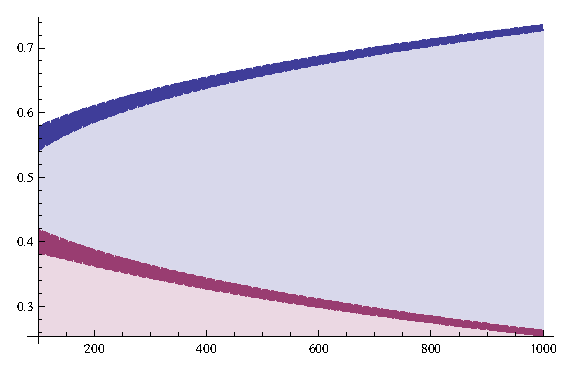
\includegraphics[width=0.6\textwidth]{figures/concorcetjury.eps}
  \caption{陪审团做出正确决定的概率}\label{fig:concorcetjury}
\end{figure}

孔多赛陪审团定理的不足之处在于其假设过于理想,比如陪审员或者投票人每个人的价值观念都不同,由于相互影响,可能更多的是以团体形式进行表决或投票,因此独立性假设与等概率假设就站不住脚;此外,在投票理论中,候选人不能通过简单的优化理论做出评价,从而难以选择出“最佳”候选人;当投票人不同、候选人得票率不同的情况下,利用简单的多数投票准则并不能得到满意的结果,即出现投票分割问题。

孔多塞方法是一类方法,我们下面介绍几个典型的孔多塞方法:柯普兰方法、凯梅尼─杨格方法、最小最大法、南森方法、道奇森方法、排名序方法和舒尔茨方法,并分析各自的性质。

\begin{definition}[孔多塞准则]
对于任意的$\mathcal A$及偏好集$\Pi[\mathcal A, \mathcal M]$,如果候选人$x\in \mathcal A$是一个孔多塞赢家,则$x$是$\mathcal F$在偏好集$\Pi[\mathcal A,\mathcal M]$上的社会选择,并且是唯一的社会选择,则称社会选择函数$\mathcal F$满足孔多塞准则或孔多塞赢家准则(Condorcet Winner Criterion,CWC)。
\end{definition}

\subsubsection{柯普兰方法}
柯普兰方法(Copeland method)是一种孔多塞方法,它利用某个候选人在和其他候选人一对一循环对决中胜出局数与落败局数之差,换而言之是其所击败的候选人数目减去将其击败的候选人数目,作为其投票分值,即
\begin{equation}\label{eq:copeland}
    V_x = \big|\{y\in \mathcal A\mid x\succ_\Pi^\mathcal{F'} y\}\big| - \big|\{y\in \mathcal A\mid y\succ_\Pi^\mathcal{F'} x\}\big|, \forall x\in \mathcal A,
\end{equation}
最终投票分值最高的候选人胜出,其中$\mathcal{F'}$表示多数投票法。根据柯普兰方法,例子\ref{eg:1980usny}中三名候选人的得分是$V_H=2$,$V_D=0$,$V_J=-2$。

柯普兰方法属于零和博弈(zero sum game):候选人Holtzman是孔多塞赢家,将其他两个候选人D'Amato和Javits悉数击败,而Javits则是孔多塞输家
(Condorcet loser),在与其他两名候选人对决时皆落败。根据柯普兰得分,孔多塞赢家Holtzman胜出,并且社会偏好为$H\succ D\succ J$。

\subsubsection{凯梅尼─杨格方法}
凯梅尼─杨格方法(Kemeny-Young method)~\cite{kemeny1959mathematics},也称凯梅尼规则、最大似然模型,也是一种基于成对比较的投票方法。KY方法考虑每个可能的偏好排名,根据社会偏好集$\Pi[n,m]$计算各个偏好排名的分值,分值最高的排名是社会选择偏好排名。KY方法将每个个体偏好排名拆解成所有可能序对偏好,利用社会偏好集确定含有对应序对偏好的票数,将对应序对偏好的票数加和即是某个个体偏好的得分。

\begin{definition}[排名分值]
对于候选集$\mathcal A$,可以生成n(n-1)种可能的偏好序对。对于某个排名$\pi\in \Pi$,有$\pi^{-1}(1)\succ \pi^{-1}(2)\succ\cdots \succ \pi^{-1}(n)$,可抽取出n(n-1)/2种序对偏好$\pi^{-1}(i)\succ \pi^{-1}(j)$,$1\le i<j \le n$。如果个体偏好排名$\sigma\in \Pi[n,m]$包含某个序对偏好,则为其投一票,遍历偏好集可算出每个序对偏好在社会偏好集上的得票
\begin{equation}
    V(x, y) = \sum\limits_{\sigma\in \Pi[n,m]} \ind(x\succ_\sigma y), \forall x, y\in \mathcal A,
\end{equation}
则排名$\pi$的分值等于其上所有可能的偏好序对的得票之和
\begin{equation}
    V_\pi = \sum\limits_{x\succ_\pi y} V(x,y) = \sum\limits_{x,y\in \mathcal A} \bigg[\ind(x\succ_\pi y) \sum\limits_{\sigma\in \Pi[n,m]} \ind(x\succ_\sigma y)\bigg].
\end{equation}
\end{definition}

\begin{definition}
凯梅尼─杨格方法是搜索$\Pi$选择出排名分值最大的偏好排名,即解如下形式的优化模型
\begin{equation}\label{eq:kemeny-youngmethod}
    \pi_\mathcal F = \argmax\limits_{\pi\in \Pi} V_\pi.
\end{equation}
最优排名$\pi_\mathcal F$中排名最高的候选人$\pi_\mathcal F^{-1}(1)\in \mathcal A$是社会偏好集$\Pi[n,m]$上的社会选择。
\end{definition}

\begin{theorem}\label{th:kemeny-young-borda}
凯梅尼─杨格方法等价于从$\Pi$搜索一个与社会偏好集$\Pi[n,m]$内所有个体偏好最近的偏好排名$\pi_\mathcal F$,以尽可能和所有选民的个人偏好保持一致。
\begin{equation}\label{eq:kemeny-young-borda}
    \pi_\mathcal F = \argmin\limits_{\pi\in \Pi} \sum\limits_{\sigma \in \Pi[n,m]} \tau(\pi,\sigma),
\end{equation}
其中,$\tau$表示肯德尔距离度量公式。
\end{theorem}

\begin{example}
根据例子\ref{eg:1980usny},我们可以构建序对偏好计票表与排名分值分布表\ref{tbl:preferencescore}。对于偏好排名$D\succ H\succ J$,其分值是$D\succ H$、$D\succ J$和$H\succ J$三个序对偏好分值之和$V_{D\succ H\succ J}$=\text{49+60+66=175}。根据偏好排名的分值可知社会选择是孔多塞赢家Holtzman,社会偏好排名是$H\succ D\succ J$,而排名分值最低的偏好排名是$J\succ D\succ H$,恰好是社会偏好排名的完全逆排列。为了验证定理\ref{th:kemeny-young-borda},我们计算所有偏好列表对的肯德尔距离以及每个个体偏好排名与社会偏好集$\Pi[n,m]$的肯德尔距离,如表\ref{tbl:preferencedistancematrix}所示,表的末行数据是根据公式\ref{eq:kemeny-young-borda}计算得到的肯德尔距离之和,其他行数据表示对应行偏好列表与列偏好列表之间的肯德尔距离。比如个体偏好$H\succ J\succ D$ 与$J\succ D\succ H$的肯德尔距离是2/3,而$J\succ D\succ H$与社会偏好集的肯德尔距离
\[
    \tau(J\succ D\succ H, \Pi[n,m]) = 2/3\times 22 + 1/3\times 23 + 1\times 15 + 2/3\times 29 + 0\times 4 + 1/3\times 7 = 177/3
\]
最大,而$H\succ D\succ J$与社会偏好集的肯德尔距离最小,式\ref{eq:kemeny-youngmethod}和\ref{eq:kemeny-young-borda}的等价性得到实例验证。
\begin{table}[ht]
    \centering
    \begin{minipage}[t]{0.33\linewidth}
    \centering
    \begin{tabular}{c|ccc}
      \hline
       & $D$ & $H$ & $J$\\
      \hline
      $D$ & -- & 49 & 60\\
      $H$ & 51 & -- & 66\\
      $J$ & 40 & 34 & -- \\
      \hline
    \end{tabular}
    \end{minipage}
    \begin{minipage}[t]{0.65\linewidth}
    \centering
    \begin{tabular}{c|c|c|c}
      \hline
      偏好排名 & 排名分值 & 偏好排名 & 排名分值\\
      \hline
      $D\succ H\succ J$ & 175 & $D\succ J\succ H$ & 143\\ %49+60+66,60+49+34
      \textbf{$H\succ D\succ J$} & \textbf{177} & $H\succ J\succ D$ & 157\\ %51+66+60,66+51+40
      $J\succ D\succ H$ & 123 & $J\succ H\succ D$ & 125\\ %40+34+49,40+34+51
      \hline
    \end{tabular}
    \end{minipage}
    \caption{序对偏好计票表(左)与偏好排名分值分布表(右)}
    \label{tbl:preferencescore}
    \vspace{0.2cm}
    \begin{minipage}[t]{0.98\linewidth}
    \centering
    \begin{tabular}{c|cccccc}
      \hline
      & \small{$D\succ H\succ J$} & \small{$D\succ J\succ H$} & \small{$H\succ D\succ J$} & \small{$H\succ J\succ D$} & \small{$J\succ D\succ H$} & \small{$J\succ H\succ D$}\\
      \hline
      \small{$D\succ H\succ J$} & 0 & 1/3 & 1/3 & 2/3 & 2/3 & 1\\
      \small{$D\succ J\succ H$} & 1/3 & 0 & 2/3 & 1 & 1/3 & 2/3\\
      \small{$H\succ D\succ J$} & 1/3 & 2/3 & 0 & 1/3 & 1 & 2/3\\
      \small{$H\succ J\succ D$} & 2/3 & 1 & 1/3 & 0 & 2/3 & 1/3\\
      \small{$J\succ D\succ H$} & 2/3 & 1/3 & 1 & 2/3 & 0 & 1/3\\
      \small{$J\succ H\succ D$} & 1 & 2/3 & 2/3 & 1/3 & 1/3 & 0\\
      \hline
      $\tau(\pi,\Pi[n,m])$ & 125/3 & 157/3 & \textbf{123/3} & 143/3 & 177/3 & 175/3\\
      \hline
    \end{tabular}
    \end{minipage}
    \caption{偏好排名肯德尔距离矩阵}
    \label{tbl:preferencedistancematrix}
\end{table}
\end{example}

KY方法是一个NP-Hard问题~\cite{bartholdi1989voting},需要遍历整个偏好排名空间$\Pi$,难以直接优化求解。可以证明,KY方法与其他几种方法之间存在紧密联系:它是孔多塞方法的最大似然估计~\cite{young1995optimal},并且还与波达计数法对赢家和输家持有完全一致的偏好~\cite{saari2000geometric}。

\section{位置筛选法}
\subsection{单记可让渡投票制}
\textbf{单记可让渡投票制}(single transferable voting,STV),肇始于19世纪50年代,由英国的Thomas Hare和丹麦的George Andrae发明,用以选出唯一的赢家。

1871年美国建筑师威廉·罗伯特·威尔William Robert Ware提出\textbf{排序复选制}(instant-runoff voting,IRV),也称\textbf{选择投票制}(alternative voting)或\textbf{偏好投票制}(preferential voting),1918年始澳大利亚众议院选举、2010年奥斯卡最佳影片的评选都采纳了IRV方法。IRV方法统计候选人的第一票数(first choice \textit{or} first preference),任何候选人只要第一票数超出半数则胜出,选举结束;否则,将第一票数最低的候选人剔除,所有含有此候选人的偏好列表也要做剔除处理,重新统计第一票数,依次类推,直至有候选人以超过半数胜出。显然,IRV是STV的一个特例。

\section{概率模型法}
\subsection{马洛斯模型}
\textbf{马洛斯模型}(Mallows Model)是一种基于距离的排名聚合方法,它利用排列空间$\Pi[n]$上定义的距离度量指标,比如肯德尔距离、斯皮尔曼距离等,确定排列空间上的概率分布。假设初始排列(location permutation)为$\sigma$,对任意的排列$\pi\in \Pi[n]$,马洛斯模型定义如下形式的概率分布
\begin{equation}\label{eq:mallowsmodel}%parametric location-spread model
    P(\pi|\sigma; c) = \frac{\exp\{-c\times d(\pi, \sigma)\}}{\sum\limits_{\pi' \in \Pi[n]} \exp\big\{-c \times d(\pi', \sigma)\big\}},
\end{equation}
其中参数$c>0$称作\textbf{离散因子}(disperse),用以控制排列空间上的距离权重。根据模型定义,构建排列空间上的概率分布需要遍历整个空间,其计算复杂度高达$\complex(n!)$,以致于无法实际应用。

\subsection{瑟斯顿模型与TrueSkill排名}%\subsection{XBox评分和TrueSkill排名}

\subsection{布雷德利─特里─卢斯模型}%Bradley–Terry–Luce

\subsection{普拉基特─卢斯模型}
\textbf{普拉基特─卢斯模型}(Plackett-Luce model,也称“卢斯模型”,简称PL模型)是一种分步排名方法,假设每个参与排名的对象都对应一个隐性分值$z$,利用隐性分值评估$\Pi[n]$的分布概率。如果决策者根据某种准则产生一个排列$\pi$,则对象$\pi^{-1}(i)$在排列$\pi$中排到第$i$位的概率$P_i$,依赖于其自身的评分$z_{\pi^{-1}(i)}$,以及其他所有排名在它下面的其他所有对象的评分之和$\sum\limits_{i\le k\le n} z_{\pi^{-1}(k)}$。PL模型对每个评分统一作单调变换,有如下形式的定义
\[
    P_i = \frac{\exp(z_{\pi^{-1}(i)})}{\sum\limits_{i\le k\le n} \exp(z_{\pi^{-1}(k)})}, 1\le i \le n.
\]
根据独立性假设,则由隐性评分列表生成排列$\pi$的概率为
\begin{equation}\label{eq:luce}
    P(\pi) = \prod\limits_{i=1}^n P_i = \prod\limits_{i=1}^n\frac{\exp(z_{\pi^{-1}(i)})}{\sum\limits_{i\le k\le n} \exp(z_{\pi^{-1}(k)})}.
\end{equation}

如果计算排列$\pi$的生成概率,只考虑位置靠前的对象评分信息,排名靠后的对象评分信息直接忽略掉,实际上对于概率评估影响甚微。比如,只考虑前$K$个位置上的对象评分信息,可以计算生成排列$\pi$的近似生成概率$P(\pi;K)$,则有定义
\begin{equation}\label{eq:luce-topk}
    P(\pi; K) = \prod\limits_{i=1}^K \frac{\exp(z_{\pi^{-1}(i)})}{\sum\limits_{i\le k\le n}\exp(z_{\pi^{-1}(k)})} \ge P(\pi),
\end{equation}
这个概率称作$n$个对象排列的\textbf{TopK概率}。当$K=n-1$时,由于$P_n = 1$,则有
\[
    P(\pi;n-1)=P(\pi;n)=P(\pi).
\]
当$K=1$时有
\begin{equation}\label{eq:luce-top1}
    P(\pi; 1) = \frac{\exp(z_{\pi^{-1}(i)})}{\sum\limits_{i\le k\le n}\exp(z_{\pi^{-1}(k)})}.
\end{equation}
如果记$n$个对象生成的所有排列集合为$\Pi[n]$,我们可以建立$P(\pi)$与$P(\pi,K)$二者之间的联系:
\begin{equation}\label{eq:luce-and-topk}
    P(\pi; K) = \sum\limits_{\sigma\in \Pi[n,K,\pi]} P(\sigma).
\end{equation}

\begin{example}
假设四个对象$\{1,2,3,4\}$存在隐性分值$Z=\{0.5, 0.8, 0.3, 0.1\}$,随机排列可以生成$4!=24$种可能的结果,如图\ref{fig:permprob-kendall}所示的多面体,每个定点对应一个排列,根据卢斯模型可以计算生成各个排列的概率。如表\ref{tbl:permuprob}所示,所有排列概率之和等于$1$,排列$\pi=\langle 1,2,3,4 \rangle$的概率$P(\pi)= 0.068102079$,排列$\pi=\langle 2,1,4,3 \rangle$的概率$P(\pi)=0.063594464$。如果根据隐性分值进行排名,可以得到最理想的排列$\pi=\langle 2,1,3,4 \rangle$,其概率最大$P(\pi)= 0.07767445$,对应图\ref{fig:permprob-kendall}中最大节点,最不理想的排列是$\pi=\langle 4,3,1,2\rangle$,其概率最小$P(\pi)=0.019200285$,对应图\ref{fig:permprob-kendall}中最小节点。

\begin{figure}[htbp]
  \centering
  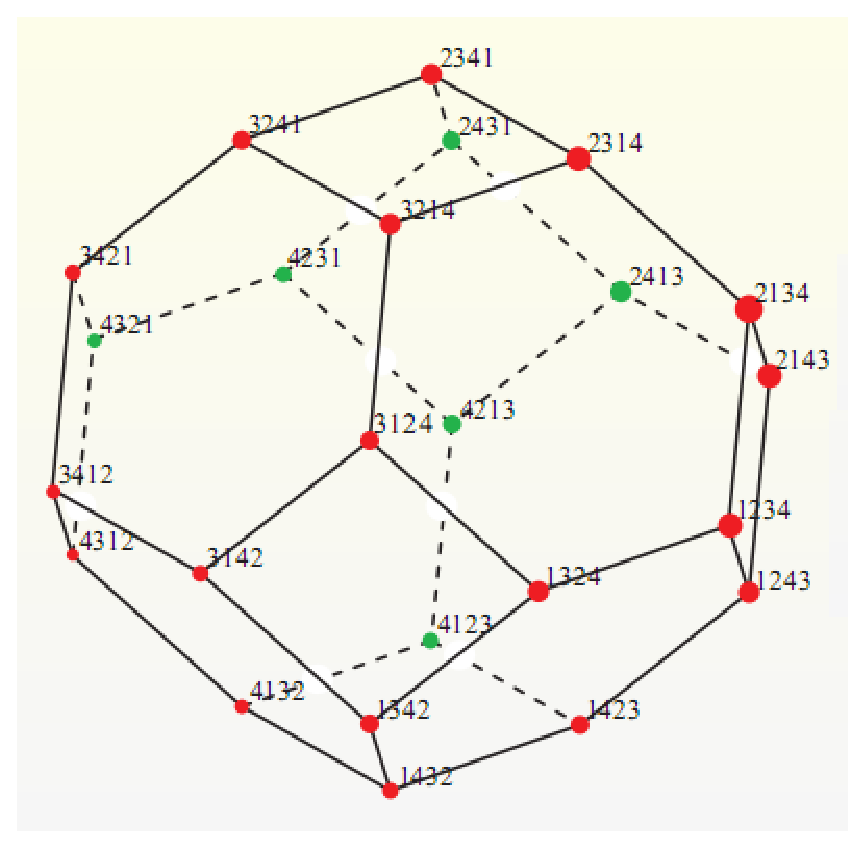
\includegraphics[width=0.5\textwidth, height=7cm]{figures/permprob-kendall.eps}\\
  \caption{排列分布及分布肯德尔距离,$1234 \triangleq \langle 1,2,3,4 \rangle$}\label{fig:permprob-kendall}
\end{figure}

\begin{table}[htbp]
    \centering
    \begin{tabular}{|c|c|c|c|c|c|c|}
\hline
$\pi$ & $\langle 1,2,3,4\rangle$ & $\langle 1,2,4,3\rangle$ & $\langle 1,3,2,4\rangle$ & $\langle 1,3,4,2\rangle$ & $\langle 1,4,2,3\rangle$ & $\langle 1,4,3,2\rangle$\\
$P(\pi)$ & 0.068102079 & 0.055757275 & 0.05019727 & 0.024927228 & 0.038285447 & 0.023221297\\
\hline
$\pi$ & $\langle2,1,3,4\rangle$ & $\langle2,1,4,3\rangle$ & $\langle2,3,1,4\rangle$ & $\langle2,3,4,1\rangle$ & $\langle2,4,1,3\rangle$ & $\langle2,4,3,1\rangle$\\
$P(\pi)$ & \bf{0.07767445} & 0.063594464 & 0.069244944 & 0.046416276 & 0.052066751 & 0.042628653\\
\hline
$\pi$ & $\langle3,1,2,4\rangle$ & $\langle3,1,4,2\rangle$ & $\langle3,2,1,4\rangle$ & $\langle3,2,4,1\rangle$ & $\langle3,4,1,2\rangle$ & $\langle3,4,2,1\rangle$\\
$P(\pi)$ & 0.047184467 & 0.023431114 & 0.057067546 & 0.038253525 & 0.020143783 & 0.027191263\\
\hline
$\pi$ & $\langle4,1,2,3\rangle$ & $\langle4,1,3,2\rangle$ & $\langle4,2,1,3\rangle$ & $\langle4,2,3,1\rangle$ & $\langle4,3,1,2\rangle$ & $\langle4,3,2,1\rangle$\\
$P(\pi)$ & 0.03430199 & 0.020805209 & 0.040900468 & 0.033486473 & \bf{0.019200285} & 0.025917675\\
      \hline
    \end{tabular}
    \caption{排列分布表}
    \label{tbl:permuprob}
\end{table}

根据定义,Top-2的排列分布(表\ref{tbl:permuprob-top1-2})可通过Top-3的排列分布计算,比如$\langle 1,2,*,*\rangle$的概率等于$\langle 1,2,3,4\rangle$ 与$\langle 1,2,4,3\rangle$ 的概率之和,即有
\[
\begin{array}{lcl}
    P(\langle 1,2,3,4\rangle) + P(\langle 1,2,4,3\rangle) & = &  0.068102079 + 0.055757275\\
    & = & P(\langle 1,2,*,*\rangle) = 0.123859355.
\end{array}
\]
Top-1排列分布(表\ref{tbl:permuprob-top1-2})可以通过Top-2的排列分布进行计算,如$\langle 3,*,*,*\rangle$的概率又等于$\langle 3,1,*,*\rangle$、$\langle 3,2,*,*\rangle$和$\langle 3,4,*,*\rangle$ 的概率之和,即有
\[
\begin{array}{lcl}
    P(\langle 3,1,*,*\rangle) + P(\langle 3,2,*,*\rangle) + P(\langle 3,4,*,*\rangle)& = & 0.070615583 + 0.095321069 + 0.047335044 \\
    & = & P(\langle 3,*,*,*\rangle) = 0.2133.
\end{array}
\]

\begin{table}[htbp]
    \centering
    \begin{tabular}{|c|c|c|c|c|c|c|}
      \hline
       $\pi; 2$ & $\langle 1,2,*,*\rangle$ & $\langle 1,3,*,*\rangle$ & $\langle 1,4,*,*\rangle$ & $\pi;1$ & $\langle 1,*,*,*\rangle$\\
       $P(\pi; 2)$ & 0.123859355 & 0.075124501 & 0.061506748 & $P(\pi; 1)$ & 0.2605\\
      \hline
       $\pi; 2$ & $\langle 2,1,*,*\rangle$ & $\langle 2,3,*,*\rangle$ & $\langle 2,4,*,*\rangle$ & $\pi;1$ & $\langle 2,*,*,*\rangle$\\
       $P(\pi; 2)$ & 0.141268922 & 0.11566122 & 0.094695399 & $P(\pi; 1)$ & 0.3516\\
      \hline
       $\pi; 2$ & $\langle 3,1,*,*\rangle$ & $\langle 3,2,*,*\rangle$ & $\langle 3,4,*,*\rangle$ & $\pi;1$ & $\langle 3,*,*,*\rangle$\\
       $P(\pi; 2)$ & 0.070615583 & 0.095321069 & 0.047335044 & $P(\pi; 1)$ & 0.2133\\
      \hline
       $\pi; 2$ & $\langle 4,1,*,*\rangle$ & $\langle 4,2,*,*\rangle$ & $\langle 4,3,*,*\rangle$ & $\pi;1$ & $\langle 4,*,*,*\rangle$\\
       $P(\pi; 2)$ & 0.055107202 & 0.074386937 & 0.045117957 & $P(\pi; 1)$ & 0.1746\\
      \hline
    \end{tabular}
    \caption{Top-2与Top-1排列分布表}
    \label{tbl:permuprob-top1-2}
\end{table}
\end{example}

\subsection{Elo排序系统}
\subsection{Colley方法}
\subsection{Massey方法}

由于地理、文化等社会人文环境的差异,世界范围内已经诞生数量可观的社会选择方法。为了分析各种方法,便于对其区分和归类,人们提出一系列性质良好的投票系统准则,如多数准则(majority criterion)、孔多塞一致性准则(Condorcet consistency)等单赢家投票系统准则。我们使用一个小节专门来介绍它们。

\section{投票系统准则}
\begin{definition}[多数准则]
如果半数以上的选民选择(或偏好)某个候选人,则此人一定是社会选择。
\end{definition}

\begin{corollary}
孔多塞方法、IRV方法、Bucklin方法和多数投票方法都满足多数准则。
\end{corollary}

\begin{definition}[孔多塞准则]
如果存在一个候选人,在和其他候选人的一对一循环对决中总能胜出,则此候选人必然胜出。
\end{definition}

\begin{corollary}
如果一个单赢家投票系统满足孔多塞准则,则它必然也满足多数准则。
\end{corollary}

\begin{corollary}
布莱克方法、柯普兰方法、道奇森方法、凯梅尼─杨格方法、最小最大法、南森方法、有序对方法(ranked pairs)和舒尔茨方法都满足孔多塞准则。
\end{corollary}

\begin{definition}[一致性准则]
假设将社会偏好集$\Pi[n,m]$任意分割成两个或多个子集,使得某个候选人$x\in \mathcal A$是每个社会偏好子集上的社会选择,如果$x$也是$\Pi[n,m]$上的社会选择,则称对应社会选择函数满足一致性准则(consistency criterion)或可分性准则(separability criterion)。
\end{definition}

\begin{corollary}
如果一个排序投票系统(ranked voting system)满足一致性,当且仅当它也是一个位置投票系统(positional voting system)。波达方法满足一致性,但柯普兰方法、IRV方法、凯梅尼─杨格方法、最小最大法、有序对方法(ranked pairs)和舒尔茨方法都违反一致性准则。
\end{corollary}

\begin{definition}[排名一致性准则]
假设将社会偏好集$\Pi[n,m]$任意分割成两个或多个子集,使得某个排序$\pi\in \Pi[n]$是每个社会偏好子集上的社会选择排序,如果$\pi$也是$\Pi[n,m]$上的社会选择排序,则称对应社会选择函数满足排名一致性准则(ranking consistency criterion)。
\end{definition}

\begin{corollary}
凯梅尼─杨格方法满足排名一致性准则。
\end{corollary}

\section{阿罗不可能定理}
1951年,美国经济学家肯尼斯·阿罗Kenneth Arrow~\cite{arrow1950difficulty,arrow2012social}使用数学公理化的方法研究社会决策时,证明了一个重要的结论:如果众多的社会成员具有不同的偏好,而社会又有多种备选方案,那么在民主的制度下不可能得到令所有的人都满意的结果。换句话说,依靠简单的“少数服从多数”的投票原则,在各种个人偏好中选择出一个共同一致的顺序,无法实现。简而言之,阿罗证明“完美的投票体系是不存在的”,即声名远播的\textbf{阿罗不可能定理}(Arrow's Impossibility Theorem)或\textbf{阿罗悖论}(Arrow's Paradox)。阿罗悖论不啻于一声惊雷,对当时的政治哲学和福利经济学产生了巨大的冲击,并为阿罗摘得1972年的诺贝尔经济学奖。

%英国哲学家约翰·洛克John Locke认为“根据自然和理性的法则,大多数具有全体的权力,因而大多数的行为被认为是全体的行为,也当然有决定权了”。在现代社会,多数原则(Majority Principle)已然成为广泛认可的社会决策方法。

社会选择,在数学上表示一个建立在所有个体偏好上的函数(或映射),其性质反映了一定的价值规范,如公民权、帕累托有效、无独裁性等。社会选择最重要的问题是:能否从逻辑上协调所有这些价值规范。阿罗使用公理性的证明,向人们宣告一个不幸的消息:世上没有同时满足\textbf{个人偏好的无限制性}、\textbf{帕累托有效}
\footnote{帕累托Vilfredo Pareto(1848~1923),意大利经济学家和社会学家。曾在都灵大学就读,后在意大利一家大型铁路公司担任工程师,升至主管,1893年起任瑞士洛桑大学教授。在经济学和社会学两个领域做出突出贡献,1906年提出帕累托最优状态(Pareto optimal)的概念,也成帕累托有效性(Pareto efficiency),奠定了现代福利经济学的基础。他认为,只要有可能使至少一个人更富裕,而同时又能使其他人保持在原来的生活水平,社会资源分配就没有达到最佳状态。}、\textbf{非相关目标独立性}与\textbf{非独裁性}四个基本公理的社会选择函数。

\begin{definition}[个人偏好的无限制性]
如果社会选择函数$\mathcal F$允许所有逻辑上可能存在的个人偏好自由表达,则称其满足无限制性(unrestricted domain)或完整性
(universality)。
\end{definition}

\begin{definition}[帕累托有效性]
对任意$x,y\in \mathcal A$,如果所有决策者一致认定$x\succ y$,则社会偏好列表$\pi_\mathcal F$也有$x\succ y$,即$x\succ_{\Pi[n,m]}^{\mathcal F} y$,则称社会选择函数$\mathcal F$满足帕累托有效性(Pareto efficiency),也称一致同意性(unanimity)。
\end{definition}

\begin{definition}[非相关目标独立性]
对于两个社会偏好集$\Pi[n,m]=\{\pi_i\}_{i=1}^m$与$\Pi'[n,m]=\{\pi'_i\}_{i=1}^m$,$\pi_i$与$\pi'_i$对应同一个决策者,$1\le i \le m$。如果每个决策者关于$x,y\in \mathcal A$的个人偏好保持不变:
\begin{equation}
    x\succ_{\pi_i} y \Leftrightarrow x\succ_{\pi'_i} y,~~1\le i\le m,
\end{equation}
则集体关于$x,y$的社会偏好在两个社会偏好集$\Pi[n,m]$和$\Pi'[n,m]$上也不会发生变化:
\begin{equation}
    x\succ_{\Pi[n,m]}^{\mathcal F} y\Leftrightarrow x\succ_{\Pi'[n,m]}^{\mathcal F} y,
\end{equation}
此时称社会选择函数$\mathcal F$满足非相关目标独立性(Independence of Irrelevant Alternatives,IIA)。
\end{definition}

\begin{definition}[非独裁性]
对于一个决策者,如果社会选择$\mathcal F$完全等价于其个人偏好$\pi$,即
\begin{equation}
    x\succ_\pi y\Leftrightarrow x\succ_{\Pi}^{\mathcal F} y,
\end{equation}
则称其为独裁者(dictator)。如果集合$\mathcal M$中没有独裁者,则称社会选择函数$\mathcal F$满足非独裁性(non-dictatorship)。
\end{definition}

\begin{definition}[线性序]
非空集合$\mathcal A$上的二元关系$\succ$称作是\textbf{线性序}(linear ordering),如果它满足
\begin{itemize}
    \item 反对称性(anti-symmetric):对任意的$x,y\in \mathcal A$,只要$x\succ y,~y\succ x$,都有$x=y$,
    \item 传递性(transitive):对任意的$x,y,z\in \mathcal A$,只要$x\succ y,~y\succ z$,都有$x\succ z$,
    \item 完备性(complete):对任意的$x,y\in \mathcal A$,要么$x\succ y$,要么$y\succ x$。
\end{itemize}
\end{definition}

\begin{definition}[社会福利函数]
如果社会选择函数$\mathcal F: \Pi[n,m]\mapsto \Pi[n]$是$\mathcal A$上的一个线性序,则称其为线性投票规则或社会福利函数(social welfare function),而其完备性对应于个人偏好的无限制性。
\end{definition}

\begin{theorem}[阿罗不可能性定理]
如果$|\mathcal A|=n>2$,则兼具帕累托有效性、非独裁性和IIA的线性投票规则$\mathcal F$不存在。换言之,兼具帕累托有效性和IIA的线性投票规则一定存在独裁者。
\end{theorem}

我们下面详细介绍1998年诺贝尔经济学奖得主阿马蒂亚·森Amartya Sen
\footnote{阿马蒂亚·森1933年生于英属印度西孟加拉邦桑蒂克尼盖登,1953年获加尔各答大学文学学士学位,1955年前往剑桥大学攻读第二个学士学位,并于1959年在剑桥大学获得博士学位。1971年起在伦敦经济学院任教,1977年起任牛津大学经济学教授,70年代末转教于美国哈佛大学。1998年1月又返回英国剑桥大学,担任三一学院
(Trinity College,Cambridge)院长。他克服了阿罗不可能定理衍生的难题,对福利经济学基础理论做出巨大贡献。}对阿罗不可能性定理的证明思路,为此先引入决定性联盟(decisive coalition)的概念。

\begin{definition}[决定性联盟]
对于非空集合$\mathcal M_c\subset \mathcal M$,以及$x,y\in \mathcal A$,如果满足
\begin{equation}
    x\succ_{\Pi[\mathcal A, \mathcal M_c]}^{\mathcal F} y \Leftrightarrow x\succ_{\Pi[\mathcal A, \mathcal M]}^{\mathcal F} y,
\end{equation}
则称$\mathcal M_c$是决定社会选择$\mathcal F$关于$(x,y)$偏好的决定性联盟。如果对任意$x,y\in \mathcal A$,$\mathcal M_c$都是决定$\mathcal F$关于$(x,y)$偏好的决定性联盟,则称$\mathcal M_c$是$\mathcal F$的决定性联盟。如果$\mathcal M_c$是所有偏好$x$甚于$y$的决策者集合,
\end{definition}
决定性联盟可以操控社会选择,严重侵害其他社会成员的利益。如果$|\mathcal M_c|>1$,决定性联盟构成寡头,在寡头集团操控下的政治生态形成寡头政治。如果$|\mathcal M_c|=1$,决定性联盟就是独裁者。我们可以证明:如果$\mathcal F$满足帕累托有效性,则$\mathcal M$是$\mathcal F$的决定性联盟。森巧妙地利用决定性联盟,推导出阿罗不可能性定理:兼具个人偏好无限制性、帕累托有效性和IIA的线性投票规则由单点集决定性联盟所操纵,即存在独裁者。

\begin{definition}[弱决定性联盟]
给定投票规则$\mathcal F$,称非空集$G\subseteq \mathcal N$是$\mathcal F$对$(x,y)$的弱决定性联盟,若对任意排序组合$\pi$,只要$G$中的成员恰好是$x\succ y$ 的所有赞成者,则社会排序$\mathcal F(\pi)$中也有$x\succ y$,即$x\succ_\pi^{\mathcal F}y$。
\end{definition}
若$G$是$\mathcal F$对$(x,y)$的决定性联盟,则$G$也是$\mathcal F$对$(x,y)$的弱决定性联盟。反过来是否成立呢?如果$\mathcal F$满足帕累托条件和独立性条件,则反过来不仅成立,而且我们还有如下更强的结论:
\begin{lemma}
设$\mathcal{F}$是满足帕累托条件和独立性条件的线性投票规则。若$G$是$\mathcal F$对$(x,y)$的弱决定性联盟,则$G$是$\mathcal F$的决定性联盟,即$G$是$\mathcal F$对任意$(x',y')$的决定性联盟。
\end{lemma}
\begin{proof}
设$\mathcal{F}$是满足帕累托条件和独立性条件的线性投票规则。设$G$是$\mathcal F$对$(x,y)$的弱决定性联盟,任给$(x',y')$,我们证明$G$是$\mathcal F$对任意$(x',y')$的决定性联盟。不妨设$x',y'$与$x,y$均不相同(相同的情况类似可证)。任给排序组合$\pi$,使得$G$中所有成员一致认为$x'\succ y'$,只需证$x'\succ_\pi^{\mathcal F}y'$。考虑如下的排序组合$\pi'$,其中
\begin{itemize}
  \item $G$中的投票者认为:$x'\succ_\pi^{\mathcal F}y'$;
  \item $G$之外的投票者认为:$x'\succ x$,$y\succ y'$,$y\succ x$,且对$x',y'$的排序与$\pi$保持一致。
\end{itemize}
易见,$G$中中的成员恰好是$x\succ y$的所有赞成者,由于$G$是$\mathcal F$对$(x,y)$的弱决定性联盟,故$x\succ_{\pi'}^{\mathcal F}y$。由于在$\pi'$中所有人都认为$x'\succ x$且$y\succ y'$,据帕累托条件有,$x'\succ_{\pi'}^{\mathcal F}x$且$y\succ_{\pi'}^{\mathcal F}y'$,据社会排序的传递性可得,$x'\succ_{\pi'}^{\mathcal F}y'$。注意到$\pi$与$\pi'$关于$x',y'$的排序上是一样的,由独立性条件有,$x'\succ_{\pi}^{\mathcal F}y'$,证毕。现在我们可以证明下面的收缩引理了。
\end{proof}

\begin{lemma}[收缩引理]
设$\mathcal F$是满足帕累托条件和独立性条件的线性投票规则。若非单点集$G$是$\mathcal F$的决定性联盟,则$G$的某个真子集$G'$也是$\mathcal F$的决定性联盟。
\end{lemma}
\begin{proof}
由于$G$是非单点集,故可将$G$拆分成两个不相交的非空子集$G_1$和$G_2$。考虑满足如下条件的排序组合$\pi$(由于备选项超过两个,故可以做到):
\begin{itemize}
  \item $G_1$中的投票者认为:$x\succ y\succ z$;
  \item $G_2$中的投票者认为:$y\succ z\succ x$;
  \item $G$之外的投票者(如果有的话)认为:$z\succ x\succ y$。
\end{itemize}
注意到$G$中所有投票者都认为$y\succ z$,由$G$是$\mathcal F$的决定性联盟可得,$y\succ_\pi^{\mathcal F} z$。现在分别考虑两种情况(由于$\mathcal F(\pi)$是完全的,故有且仅有两种情况):
\begin{itemize}
  \item $x\succ_\pi^{\mathcal F}z$。任给排序组合$\pi'$,使得$G_1$中的成员在$\pi'$中恰好是$x\succ z$的所有赞成者,由于在$\pi$中$G_1$中的成员也恰好是 $x\succ z$的所有赞成者,故由独立性条件可得,$x\succ_{\pi'}^{\mathcal F} z$,这意味着$G_1$是$\mathcal F$对$(x,z)$的弱决定性联盟,再据引理1有,$G_1$是$\mathcal F$的决定性联盟。
  \item $z\succ_\pi^{\mathcal F}x$。此时,据$\mathcal F(\pi)$的传递性有$y\succ_\pi^{\mathcal F}x$。同理于情况1可证,$G_2$是$\mathcal F$的决定性联盟。
\end{itemize}
综上,总有$G$的真子集是决定性联盟,证毕\footnote{Logic:\href{http://www.cnblogs.com/ilogic/archive/2012/08/05/proof\_arrow.html}{阿罗不可能性定理的证明}}。
\end{proof}

\section{吉伯德-萨特思韦特定理}
19世纪80年代,投票选举理论的奠基人之一查尔斯·勒特威奇·道奇森Charles Lutwidge Dodgson
\footnote{查尔斯·勒特威奇·道奇森(1832--1898),笔名路易斯·卡罗尔Luis Carroll,英国数学家、《艾丽丝漫游奇境记》及续篇《爱丽丝镜中奇遇》的作者。他天赋异禀,在几何学、线性代数、矩阵与逻辑学面都颇有研究,写出十多本数学著作,为线性代数与概率论两大领域提供了新思路。他认为一个合理的选举规则应当在孔多赛赢家存在时始终选择孔多赛赢家,在孔多赛赢家不存在时,仍然能够选择最接近于孔多赛赢家的候选人:(孔多赛赢家不存在),他的这一思想被人称作道奇森准则。}
开始关注对投票规则的研究,认为人们在投票时的行为更倾向于策略投票。个人出于某种目的策略性的需要,通过谎报自己的真实偏好,使得决策结果往有利的方向变化。个人谎报其真实偏好,可能会造成损人不利己的后果,选出对各方均不利的候选人,对公众权利产生不利影响。为此有必要深入研究策略性投票对选举的操纵,以期设计出防止策略性投票的社会选择方法。

如果在投票选举时存在策略性投票,个人所表达的偏好偏离其真实偏好,研究学者有理由重新审视阿罗不可能定理。20世纪70年代密歇根大学的阿兰·吉伯德Allan Gibbard 和西北大学的马克·萨特思韦特Mark Satterthwaite分别独立提出两个几乎相同的定理,统称\textbf{吉伯德-萨特思韦特定理}(Gibbard--Satterthwaite Theorem)防策略投票的不可能性定理,引起数学、经济学、计算机科学和哲学等诸多领域学者的广泛关注。

\begin{definition}[战略免疫性]
如果其他个体均真实披露自己偏好信息,某个特定个体只有真实显示自己的偏好时社会选择对自己才最有利,则称对应社会选择规则可免于战略性投票操纵
(non-manipulable),即具有\textbf{战略免疫性}(strategy-proofness)。
\end{definition}

\begin{theorem}[吉伯德-萨特思韦特定理]
在社会选择规则集合内不存在同时满足个人偏好无限制性、帕累托有效性、非独裁性、传递性和战略免疫性五个基本公理的选择规则。
\end{theorem}
根据吉伯德─萨特思韦特定理,我们意识到非独裁性和战略免疫性两个属性可能存在内在矛盾,任何合理的社会选择规则都难以两面兼顾:在所有可能的社会选择规则下,能够同时满足个人偏好无限制性、帕累托有效性、传递性和战略免疫性的只有独裁规则。如果存在一个社会选择规则兼具个人偏好无限制性、帕累托有效性、非独裁性和传递性,则它必定无法免于战略性投票操纵。

许多社会选择方法满足一系列良好的公理性质,但是却免不了受到战略性投票的操控,总是存在隐瞒自己真实偏好的个体,试图取得对自己有利的选举局面。人们无法设计出一个确保或诱使所有个体能够道出其真实偏好(revelation principle)的社会选择机制。人们只能另辟蹊径,将目光转移到社会选择战略性操纵复杂度的研究,通过增加战略性投票操纵的成本,以降低人们投出违心选票的动机,比如20世纪90年代乔治亚理工学院教授约翰·巴托尔迪三世John Bartholdi III等人\cite{bartholdi1989computational,bartholdi1989voting}的卓越工作,促进了计算社会选择的快速发展:以高计算复杂度阻止策略性投票操纵,间接地迫使个体对其偏好做出真实的回应。由于选举操纵能够抑制部分个体耍诈,已然成为衡量一个社会选择准则优劣性的一个指标。

\section{梅定理}
\begin{definition}[匿名性]
如果集体选择的结果只依赖于各个个体的偏好与决策,与特定决策由具体谁做出无关,则称此集体选择具备\textbf{匿名性}(anonymity),或称决策者是对称主体。
\end{definition}

\begin{definition}[中立性]
如果决策规则在任意两个备选对象之间中立,则称它满足\textbf{中立性}(neutrality)。对于线性序形式的偏好排名,对于$m$个备选对象,存在$m!$种偏好排名,如果决策者的数目是$n$,则所有决策者可能产生的偏好排名组合有$m!^n$个。对于任意一个排名排名组合$P$,决策规则$r$的选择$r(P)=c$,对所有偏好排名组合$P$所含的所有偏好排名施加相同的排列运算$M$,如果决策规则选择$r(M(P))=M(r(P))$,则称它满足中立性。
\end{definition}

\begin{definition}[正向响应]
正向响应(positively responsive)
\end{definition}

\begin{theorem}[梅定理May's Theorem]
在集体选择的备选对象是二元的情况下,一种集体决策规则是简单多数规则,当且仅当它满足匿名性、中立性和正向响应。
\end{theorem}

%\section{Manipulations of Voting}

\section{排名聚合}
\textbf{排名聚合}(rank aggregation),也称\textbf{数据融合}(data fusion),源于投票选举问题,通过融合多个来源的对象排名结果,从而更加准确地反映对象间的优先等级秩序。目前,排名聚合已经在网络信息检索、统计检验、体育竞技排名等多个领域得到广泛应用,比如元搜索引擎接收用户提交的检索词,同时向多个基本搜索引擎的发送检索请求,将多个基本搜索引擎的搜索结果聚合而形成最终结果反馈给用户。

排名聚合的目标是从$\Pi[n]$中搜索一个理想的排列$\hat\pi$,使得它和所有已知排名列表$\{\pi_1,\pi_2,\ldots\}$保持尽可能的一致,数学上等价于解一个优化问题:
\begin{equation}\label{eq:rankaggregationproblem}
    \hat\pi = \argmax\limits_{\pi\in \Pi[n]} \sum\limits_i s(\pi,\pi_i) = \argmin\limits_{\pi\in \Pi[n]} \sum\limits_i d(\pi,\pi_i),
\end{equation}
其中$s(\pi,\sigma)$是衡量两个排名列表$\pi$和$\sigma$之间的相似性指标,$d(\pi,\sigma)$是由相似性指标$s(\pi,\sigma)$导出的某种距离度量,如肯德尔Tau。

\begin{table}[htbp]
\centering
\begin{tabular}{|c|l|c|l|}
\hline
编号 & 网址 & 编号 & 网址\\
\hline
1 & abcnews.go.com/health & 8 & www.cnn.com/HEALTH\\
2 & en.wikipedia.org/wiki/Health & 9 & www.health.com\\
3 & en.wikipedia.org/wiki/Health\_care & 10 & www.mayoclinic.com\\
4 & health.yahoo.net & 11 & www.nytimes.com/pages/health/\\
5 & health.gov & 12 & www.pacificprime.com\\
6 & reuters.com/news/health & 13 & www.webmd.com\\
7 & wiki.ask.com/Health &&\\
\hline
\end{tabular}
\caption{九个搜索引擎检索关键词“health”的十三条搜索结果}
\label{tbl:metaserp}
\end{table}

\begin{table}[htbp]
\centering
\begin{tabular}{|l|c|l|c|l|c|}
\hline
搜索引擎 & 搜索结果 & 搜索引擎 & 搜索结果 & 搜索引擎 & 搜索结果\\
\hline
AOL & $\langle 9,13,10,2,8\rangle$ & Bing & $\langle 2,13,4,5,11\rangle$ & DuckDuckGo & $\langle 4,13,2,1,6\rangle$ \\
Excite & $\langle 13,2,11,4,8\rangle$ & Google & $\langle 2,3,9,4,12\rangle$ & HotBot & $\langle 2,13,4,8,10\rangle$ \\
Lycos & $\langle 2,13,4,8,10\rangle$ & Teoma & $\langle 9,13,10,7,8\rangle$ & Yahoo! & $\langle 13,2,4,8,10\rangle$\\
\hline
\end{tabular}
\caption{九个搜索引擎检索关键词“health”的前5条搜索结果}
\label{tbl:serplist}
\end{table}

\begin{example}\label{eg:metasearch}
人们在使用搜索引擎检索信息时,比如提交检索词“health”,不同搜索引擎搜索并返回的结果通常也不相同。目前,正常提供服务的搜索引擎不下于1,000个。2011年10 月22 日,我们使用9个搜索引擎:
\underline{A}OL、\underline{B}ing、\underline{D}uckDuckGo、\underline{E}xcite、\underline{G}oogle、\underline{H}otBot、\underline{L}ycos、
\underline{T}eoma和\underline{Y}ahoo!,分别检索关键词“Health”,提取每个搜索引擎的前5条搜索条目汇集成13条搜索结果,如表\ref{tbl:metaserp}所示根据字母顺序为搜索条目对应网址编号,表\ref{tbl:serplist}是每个搜索引擎前5条搜索条目的排列结果。根据波达计数法则对搜索条目进行评分,如表\ref{tbl:bordarank}所示,第2 列至第14列是各个搜索引擎在对应搜索条目上的评分,聚合排名的结果是
\[
    \pi = \langle 13,2,4,8,10,9,11,3,1/5/7,6/12\rangle,
\]
其中$a/b$表示$a$和$b$评分相同,无法区分。如果我们预先对各个搜索引擎设定一个权值,比如
\[
\begin{array}{lcccccccccl}
    \omega &= &\{\omega_A,& \omega_B, & \omega_D & \omega_E, & \omega_G, & \omega_H, & \omega_L,&\omega_T, & \omega_Y\} \\
    &= & \{0.80, & 0.98, & 0.80, & 0.80, & 1.00, & 0.85, & 0.85, & 0.88, & 0.95\},
\end{array}
\]
重新计算加权评分,则有聚合排名结果
\[
    \pi_\omega = \langle 2,13,4,8,10,9,11,3,5,12,7,1,6\rangle.
\]
\end{example}
\begin{table}[htbp]
\centering
\begin{tabular}{|l|c|c|c|c|c|c|c|c|c|c|c|c|c|}
\hline
Rank & 1 & 2 & 3 & 4 & 5 & 6 & 7 & 8 & 9 & 10 & 11 & 12 & 13\\
\hline
A (0.80) &  & 10 &  &  &  &  &  & 9 & 13 & 11 &  &  & 12\\
B (0.98) &  & 13 &  & 11 & 10 &  &  &  &  &  & 9 &  & 12\\
D (0.80) & 10 & 11 &  & 13 &  & 9 &  &  &  &  &  &  & 12\\
E (0.80) &  & 12 &  & 10 &  &  &  & 9 &  &  & 11 &  & 13\\
G (1.00) &  & 13 & 12 & 10 &  &  &  &  & 11 &  &  & 9 &  \\
H (0.85) &  & 13 &  & 11 &  &  &  & 10 &  & 9 &  &  & 12\\
L (0.85) &  & 13 &  & 11 &  &  &  & 10 &  & 9 &  &  & 12\\
T (0.88) &  &  &  &  &  &  & 10 & 9 & 13 & 11 &  &  & 12\\
Y (0.95) &  & 12 &  & 11 &  &  &  & 10 &  & 9 &  &  & 13 \\
\hline
TS & 10 & 97 & 12 & 77 & 10 & 9 & 10 & 57 & 37 & 49 & 20 & 9 & 98\\
\hline
WTS & 8.0 & 85.64 & 12.0 & 68.33 & 9.8 & 7.2 & 8.8 & 48.82 & 32.84 & 42.33 & 17.62 & 9.0 & 84.67\\
\hline
\end{tabular}
\caption{波达排名与加权波达排名列表:首列括号内数值是各搜索引擎的权值,TS是各条目的总得分(Total Score),WTS是各条目的加权总得分
(Weighted Total Score)。}
\label{tbl:bordarank}
\end{table}

\subsection{序对投票准则}
设有$n$个候选人$\{1,2,\ldots,n\}$,每个选民都从中选出部分候选人并排列,所有选民的排列集合记作$\Pi$。每个排列$\pi\in \Pi$反映一个选民对部分候选人的偏好,越是其喜欢的候选人在选票中的排名越靠前。我们提出一种\textbf{序对投票}(pairwise voting, PV)准则,根据所有候选人组合在$\pi$ 中的相对名次进行评分。PV准则对所有没有入选$\pi$的候选人等同视之,则有$\pi(i)=|\pi| + 1$。对于某个候选人组合$(i,j)$,我们根据如下形式的序对投票准则构建序对评分矩阵$V(\pi)\in \mathbb R^{n\times n}$:
\begin{equation}\label{eq:pvc}
    v_\pi(i,j) = \frac{\pi(j)-\pi(i)}{\min\{\pi(i),\pi(j)\}}.
\end{equation}
当$\pi(i) < \pi(j)$时,候选人$i$在$\pi$中的排名比$j$的排名靠前,则$v_\pi(i,j)>0$;当$\pi(i) > \pi(j)$时,候选人$i$在$\pi$中的排名比$j$的排名靠后,则$v_\pi(i,j)=-v_\pi(j,i) < 0$;当$v_\pi(i,j)=v_\pi(j,i)$时,则$v_\pi(i,j)=0$。由此可知,序对评分矩阵$V(\pi)$是一个反对称矩阵$V(\pi) = -V^T(\pi)$。

每个候选人对应评分矩阵$V$的一行,如果计算序对评分矩阵的行和,则可以直接确定候选人从单个选民排名列表中的综合得分。实际上,评分矩阵每个行元可以看作是一次比赛结果。如果比赛胜利,则得分为正,比赛失利则得分为负。对于任意一个候选人$i$,它从某个选民排名列表$\pi\in \Pi$获得的总分记作$V_i(\pi)$,则有
\begin{equation}
    V_i(\pi) = \sum\limits_{1\le j\le n} v_\pi(i,j) = \sum\limits_{1\le j\le n} \frac{\pi(j)-\pi(i)}{\min\{\pi(i),\pi(j)\}}.% = -[(i-1) + \frac{i-2}{2} + \ldots + \frac{1}{i-1}] + \frac{1 + \ldots + (m - i)}{i}+ (n - m) \frac{m - i + 1}{i},
\end{equation}

如果记$\mathscr P_{i*}(\pi)=\{1\le j\le n, \pi(i) < \pi(j)\}$,$\mathscr P_{*i}(\pi)=\{1\le j\le n, \pi(j) < \pi(i)\}$分别对应$\pi$中排到候选人$i$之后的候选人集合、排到候选人$i$之前的候选人集合,利用它改写上式,则有
\begin{equation}
\begin{array}{lcl}
    V_i(\pi) &=& \sum\limits_{1\le j\le n} \frac{\pi(j)-\pi(i)}{\min\{\pi(i),\pi(j)\}} =  \sum\limits_{j\in \mathscr P_{i*}(\pi)} \frac{\pi(j)-\pi(i)}{\pi(i)} + \sum\limits_{j\in \mathscr P_{*i}(\pi)} \frac{\pi(j)-\pi(i)}{\pi(j)}\\
    &=& \sum\limits_{j\in \mathscr P_{i*}(\pi)} \big[\frac{\pi(j)}{\pi(i)} -1\big] + \sum\limits_{j\in \mathscr P_{*i}(\pi)} \big[1-\frac{\pi(i)}{\pi(j)}\big],\\
    &=& \sum\limits_{\pi(i)+1\le k \le |\pi|} \big[\frac{k}{\pi(i)} -1\big] + [n-|\pi|][\frac{|\pi|+1}{\pi(i)}-1] + \sum\limits_{1\le k \le \pi(i)-1} \big[1-\frac{\pi(i)}{k}\big].
\end{array}
\end{equation}
可以证明:$V_i(\pi)$是一个关于$\pi(i)$单调不增函数。当候选人落选$\pi$,$\pi(i)=|\pi|+1$,前两部分都等于零,则有
\begin{equation}
    V_i(\pi) = |\pi| - \pi(i)\sum\limits_{1\le k \le |\pi|} \frac{1}{k}.
\end{equation}
对于排在首位的候选人$i$,$\pi(i)=1$,其分值$V_1(\pi)=m(2n-m-1)/2$。

我们根据PV准则确定每个选民排名列表产生的评分矩阵,通过行和运算获得每个候选人在各个排名列表$\pi$所得综合评分。如果累积候选人在所有选民排列上的综合评分,从而可以算得其最终投票得分
\begin{equation}\label{eq:pvagg}
    V_i = \sum\limits_{\pi\in\Pi} V_i(\pi) = \sum\limits_{\pi\in\Pi} \sum\limits_{1\le j\le n} v_\pi(i,j) = \sum\limits_{\pi\in\Pi} \sum\limits_{1\le j\le n} \frac{\pi(j)-\pi(i)}{\min\{\pi(i),\pi(j)\}}, 1\le i \le n.
\end{equation}
我们依据候选人最终投票得分进行排名。此外,如果我们拥有各个选民的权值信息$\omega$,可以对聚合评分进行加权处理,则有
\begin{equation}\label{eq:wpvagg}
    V_i = \sum\limits_{\pi\in\Pi} \omega_\pi V_i(\pi) = \sum\limits_{\pi\in\Pi} \omega_\pi \sum\limits_{1\le j\le n} \frac{\pi(j)-\pi(i)}{\min\{\pi(i),\pi(j)\}}, 1\le i \le n.
\end{equation}
\begin{table}[htbp]
\centering
\begin{tabular}{|c|c|c|c|c|c|c|c|c|c|c|c|}
\hline
& $V_i(\pi_A)$ & $V_i(\pi_B)$ & $V_i(\pi_D)$ & $V_i(\pi_E)$ & $V_i(\pi_G)$ & $V_i(\pi_H)$ & $V_i(\pi_L)$ & $V_i(\pi_T)$ & $V_i(\pi_Y)$ & $V_i$\\
\hline
1 & -8.7 & -8.7 & -0.1 & -8.7 & -8.7 & -8.7 & -8.7 & -8.7 & -8.7 & -69.68\\
\hline
2 & -0.1 & 50.0 & 6.5 & 18.0 & 50.0 & 50.0 & 50.0 & -8.7 & 18.0 & 233.72\\
\hline
3 & -8.7 & -8.7 & -8.7 & -8.7 & 18.0 & -8.7 & -8.7 & -8.7 & -8.7 & -51.60\\
\hline
4 & -8.7 & 6.5 & 50.0 & -0.1 & -0.1 & 6.5 & 6.5 & -8.7 & 6.5 & 58.43\\
\hline
5 & -8.7 & -0.1 & -8.7 & -8.7 & -8.7 & -8.7 & -8.7 & -8.7 & -8.7 & -69.68\\
\hline
6 & -8.7 & -8.7 & -4.8 & -8.7 & -8.7 & -8.7 & -8.7 & -8.7 & -8.7 & -74.42\\
\hline
7 & -8.7 & -8.7 & -8.7 & -8.7 & -8.7 & -8.7 & -8.7 & -0.1 & -8.7 & -69.68\\
\hline
8 & -4.8 & -8.7 & -8.7 & -4.8 & -8.7 & -0.1 & -0.1 & -4.8 & -0.1 & -40.80\\
\hline
9 & 50.0 & -8.7 & -8.7 & -8.7 & 6.5 & -8.7 & -8.7 & 50.0 & -8.7 & 54.30\\
\hline
10 & 6.5 & -8.7 & -8.7 & -8.7 & -8.7 & -4.8 & -4.8 & 6.5 & -4.8 & -36.25\\
\hline
11 & -8.7 & -4.8 & -8.7 & 6.5 & -8.7 & -8.7 & -8.7 & -8.7 & -8.7 & -59.22\\
\hline
12 & -8.7 & -8.7 & -8.7 & -8.7 & -4.8 & -8.7 & -8.7 & -8.7 & -8.7 & -74.42\\
\hline
13 & 18.0 & 18.0 & 18.0 & 50.0 & -8.7 & 18.0 & 18.0 & 18.0 & 50.0 & 199.30\\
\hline
$\omega$ & 0.80 & 0.98 & 0.80 & 0.80 & 1.00 & 0.85 & 0.85 & 0.88 & 0.95 &\\
\hline
\end{tabular}
\caption{序对投票准则下的搜索排名聚合}
\label{tbl:metasearch-pv}
\end{table}
我们下面使用例\ref{eg:metasearch}介绍PV准则,搜索条目$\{1,\ldots,13\}$ 对应13个候选人,9个基本搜索引擎:
\underline{A}OL、\underline{B}ing、\underline{D}uckDuckGo、\underline{E}xcite、\underline{G}oogle、\underline{H}otBot、\underline{L}ycos、
\underline{T}eoma和\underline{Y}ahoo!构成评价搜索条目9个选民,分别产生一个等长度($|\pi|=5$)的搜索排名列表:
\[
\begin{array}{lll}
    \pi_A =\langle 9,13,10,2,8\rangle, & \pi_B = \langle 2,13,4,5,11\rangle, & \pi_D = \langle 4,13,2,1,6\rangle, \\
    \pi_E = \langle 13,2,11,4,8\rangle, & \pi_G = \langle 2,3,9,4,12\rangle, & \pi_H = \langle 2,13,4,8,10\rangle, \\
    \pi_L = \langle 2,13,4,8,10\rangle, & \pi_T = \langle 9,13,10,7,8\rangle, & \pi_Y = \langle 13,2,4,8,10\rangle.
\end{array}
\]
依据PV评分准则,我们可以计算每一个搜索条目从9个排名列表得到的评分。如表\ref{tbl:metasearch-pv}所示,第9个搜索条目在Google给出的搜索排名列表中排在第3位,它从中可以得到的分值为
\[
    V_9(\pi_G) = \sum\limits_{4\le k \le 5} \big[\frac{k}{3} -1\big] + (13-5)(\frac{5+1}{3}-1) + \sum\limits_{1\le k \le 2} \big[1-\frac{3}{k}\big] = 6.5.
\]
如表\ref{tbl:metasearch-pv}最后一列所示,利用PV评分准则得到的聚合排名列表为
\[\pi = \langle 2, 13, 4, 9, 10, 8, 3, 11, 1, 5/7, 6, 12\rangle.\]
如果使用例\ref{eg:metasearch}中提供的搜索引擎权向量$\omega$(见表\ref{tbl:metasearch-pv}末行数据),可以得到加权聚合排名
\[\pi = \langle 2, 13, 4, 9, 8, 10, 3, 11, 1, 7, 5, 6, 12\rangle.\]
对比结果见图\ref{fig:pvaggregation},加权排名聚合结果是严格的不含平手项的聚合排名列表,加权结果破除了条目5和7平手的局面,调整搜索条目8与10的相对位置。如果统计9个搜索引擎的搜索排名列表可以发现,条目8排到条目10之前列表有4个,条目8排到条目10之后的只有2个,在其他列表都没有出现,加权结果似乎更加合乎事实。
\begin{figure}[ht]
    \begin{minipage}[t]{0.5\linewidth}
        \centering
          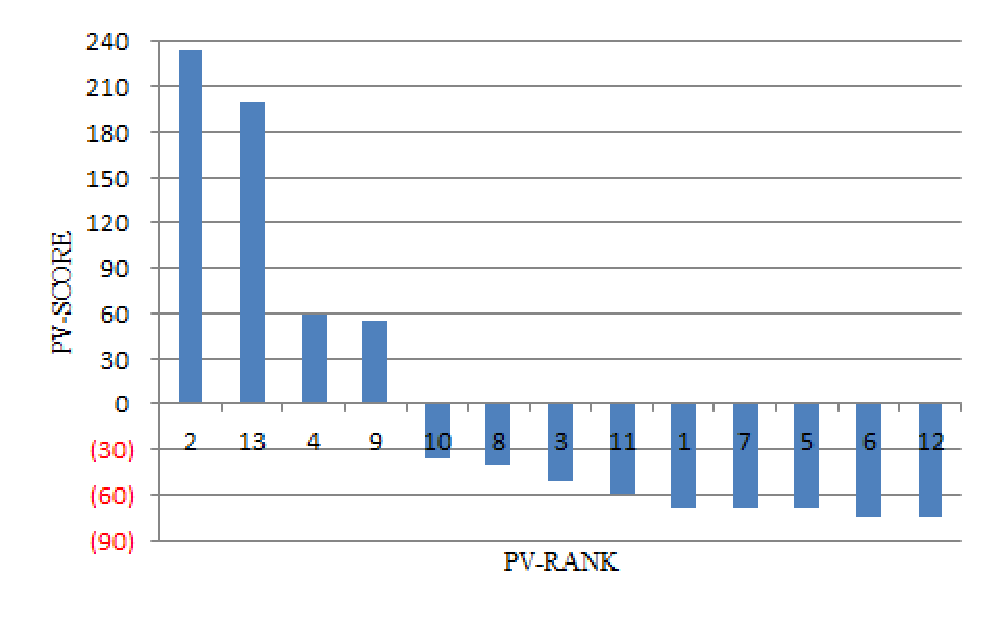
\includegraphics[width=0.99\textwidth,height=5cm]{figures/pv}
    \end{minipage}
    \begin{minipage}[t]{0.5\linewidth}
        \centering
          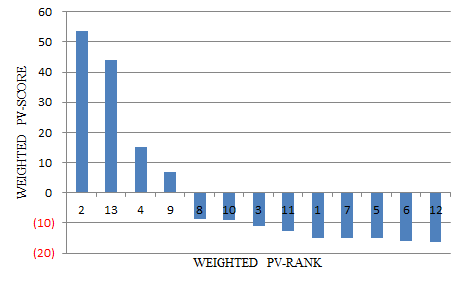
\includegraphics[width=0.99\textwidth,height=5cm]{figures/weightedpv}
    \end{minipage}\caption{序对投票准则下的搜索排名聚合(\textbf{左})与加权排名聚合(\textbf{右})}\label{fig:pvaggregation}
\end{figure}

\chapter{排名收敛}
传统数值迭代方法,如牛顿法、高斯-赛德尔方法、超松弛迭代、雅克比方法和幂法,大多根据相邻迭代结果之间偏差界作为判定迭代收敛而终止迭代计算的准则,我们称其为\textbf{数值收敛准则}(convergence in value)。

在网页搜索领域,PageRank是影响搜索引擎排名的一个重要因素,计算网页PageRank分值的方法有多种,幂法是其中应用最广泛的一种,关于PageRank的研究论文达上万篇
\footnote{根据Google Scholar搜索结果,截止2013年03月26日下午16:30,标题中包含PageRank关键词的可下载PDF文献有10,800条。},
然而绝大多数关于PageRank 分值的计算都是基于数值收敛准则。由于PageRank主要应用在网页排名,相比精确分值而言,我们更关心的是各个网页的排名顺序。

Peserico和Pretto在\cite{peserico2007does,peserico2012hits}首次正式给出迭代排名算法的\textbf{$\epsilon$-排名收敛}(convergence in rank)直观性的定义,并提出一些开放性的问题,比如数值收敛与排名收敛是否存在强关联性,链接图的类型对两种收敛准则的影响等。本文旨在解决此类开放性问题,首先从“序”的概念出发,定义一种基于序稳定性的收敛准则,再从数学上严格证明序稳定性与数值稳定性之间的联系。我们将序稳定性收敛准则应用到PageRank算法的计算,从而大幅提升网页排名计算的性能。

\begin{definition}[排列模式]%Permutation Pattern
对于一个长度为$n$的排列$\pi=\pi_1\pi_2\ldots\pi_n$,其中$\pi_i$表示排列中的第$i$个数。比如,在排列$\pi=391867452$中,$\pi_1=3$,$\pi_9=2$。如果排列$\pi$存在一个子列(不必连续)与排列$\sigma$具有相同的相对序关系,则称$\pi$包含$\sigma$,排列$\sigma$称作$\pi$的一个\textbf{模式}(pattern),并记作$\sigma\le \pi$。由于排列$\pi=391867452$中含有子列($91674, 91675, 91672$),则称它含有模式$\sigma=51342$。每个子列都称作$\sigma$的一个\textbf{复本}
(copy)或出现一次$\sigma$。由于$\pi$不包含一个长度为4的递增序列,可以说它不包含模式$1234$。
\end{definition}

\begin{definition}[序关系]
对于非空集合$A$上的二元关系$\prec$,如果
\begin{enumerate}
    \item 对任意的$a\in A$,都有$a\prec a$,则称它满足\textbf{自反性}(reflexive);
    \item 对任意的$a,b,c\in A$,只要$a\prec b,~b\prec c$,都有$a\prec c$,则称它满足\textbf{传递性}(transitive);
    \item 对任意的$a,b\in A$,只要$a\prec b,~b\prec a$,都有$a\prec a$,则称它满足\textbf{反对称性}(anti-symmetric);
    \item 对任意的$a,b\in A$,要么$a\prec b$,要么$b\prec a$,则称它满足\textbf{完备性}(complete)。
\end{enumerate}
如果二元关系$\prec$满足自反性和传递性,则称它是“\textbf{预序}”(pre-order)关系;如果还满足反对称性,则称它是“\textbf{偏序}”(partial order)关系,$A$是“偏序集”(partial order set,poset);如果还满足完备性,则称它是“\textbf{全序}”(total order)关系,也称“\textbf{线性序}”(linear order)或“\textbf{简单序}”(simple order)。
\end{definition}

%根据全序关系,非空集合可以产生唯一的线性链表。
本文在不产生混淆的情况下,使用\textbf{“序关系”}表示$n$ 维实向量,比如$u=(u_1,u_2,\ldots,u_n)^T$ 各元素(实数)之间的全序关系$\le$。
\begin{property}
实数集上的二元关系“$<$”是偏序关系,但不是全序关系;“$\le$”既是偏序也是全序关系。
\end{property}

\begin{definition}[排列]
\end{definition}

\begin{definition}[偏好关系]%preference relation, power law, small world
\end{definition}

\begin{definition}[实数排列]
对于向量$u\in \mathbb R^n$,对向量所有元素按照二元序关系$\le$进行排列,如果逐次记录所有维度上的排名序构成一个新的向量,则称它是向量$u$的“\textbf{序数列}”,记作$\pi(u)$,符号$\pi(u_i)\in \mathbb{R}$表示$u_i$的\textbf{序/排名},$\pi_i^{-1}(u)$表示向量$u$按照“序关系”排在$i$位的元素,元素的数值越小则“序”越大。假设以$u$的序数列为标准,我们称$\pi(u)$为\textbf{“理想序数列”},相应的各个元素的序为\textbf{“理想序”}。
\end{definition}

\begin{definition}[保序映射]
假设$\prec_A$和$\prec_B$分别是定义在集合$A$和$B$上的全序关系,$f:A\mapsto B$是从集合$A$到集合$B$上的一个双射,对任意的$x,y\in A$,如果$x\prec_A y$,则有$f(x)\prec_B f(y)$,那么$f$称作是从集合$A$到集合$B$的一个\textbf{保序映射}(preserving mapping)。
\end{definition}

\begin{definition}
如果向量$u,v\in \mathbb R^n$满足$\big[\pi(u_i)-\pi(u_j)\big]\big[\pi(v_i)-\pi(v_j)\big]>0,~~~\forall 1\le i\ne j\le n$,则称$u$和$v$\textbf{同序},否则称两者\textbf{逆序}。如果存在函数$f:\mathbb{R}^n \mapsto \mathbb{R}^n$,使得$f(u)$与$u$同序,则称$f$是\textbf{保序函数}。
\end{definition}

\begin{example}
对于5维向量$u=(0.2,0.1,0.6,0.5,0.3)^T$,则$0.1\le 0.2\le 0.3\le 0.5\le 0.6$,则$\pi(u)=(4,5,1,2,3)$,而$\pi(u_5)=3$,$\pi_2^{-1}(u)=0.5$。对于向量
\[
    v=(0.4,0.2,1.2,1.0,0.6)^T, ~~~w=(0.3,0.2,0.7,0.6.0.4)^T
\]
它们与$u$相互“同序”。由此可知,对于任意向量$u$,变换
\[
    \begin{array}{l}
      f:u_i \mapsto u_i + a \\
      g:u_i \mapsto \lambda u_i
    \end{array}
\]
其中,$a\in \mathbb{R}, \lambda>0$,则变换$f,g$都是保序的。
\end{example}

\begin{definition}[序距]
对于任意的$u,v\in \mathbb{R}^n$,$\pi(u),\pi(v)\in \mathbb{R}^n$,如果$\delta:\mathbb{R}^n \times \mathbb{R}^n \mapsto \mathbb{R}$满足如下性质:
\begin{enumerate}
\item 如果$u$和$v$同序,则$\delta(u,v)=0$;
\item 如果$u$和$v$逆序,将$v$中元素随机排列构成集合$V$,对任意$v_\alpha\in V$,都有$\delta(u,v)\ge \delta(u,v_\alpha)\ge 0$;
\item 如果以$\pi(u)$为理想序数列,对任意的$i<j<k$,交换元素$\pi_i^{-1}(u)$和$\pi_j^{-1}(u)$的位置(序/排名),得到$u_\beta$,交换元素$\pi_i^{-1}(u)$ 和$\pi_k^{-1}(u)$的位置,得到$u_\gamma$,保持其他元素的位置不变,则$\delta(u,u_\beta)> \delta(u,u_\gamma)$。
\end{enumerate}
则称$\delta$是$u$和$v$的\textbf{序距}(ordinal distance)。
\end{definition}

\begin{definition}[序稳定性与序收敛准则]%Rank Stability

\end{definition}

%\chapter{元搜索引擎}
%元搜索引擎(简称“元搜”)是一种“超搜索引擎”。它通过统一的搜索界面,将用户的检索请求,提交给多个搜索引擎,并将各搜索引擎返回的搜索结果经过滤重、聚类、重排等过程,展示给用户(见图\ref{fig:metase})。接收元搜索引擎检索请求的搜索引擎,称作“源搜索引擎”、“成员搜索引擎”或者“独立搜索引擎”,我们在后文统一称之为“独立搜索引擎”。一般而言,元搜没有独立的爬虫,依赖于独立搜索引擎而存在。
%
%\begin{figure}[ht]
%  \centering
%  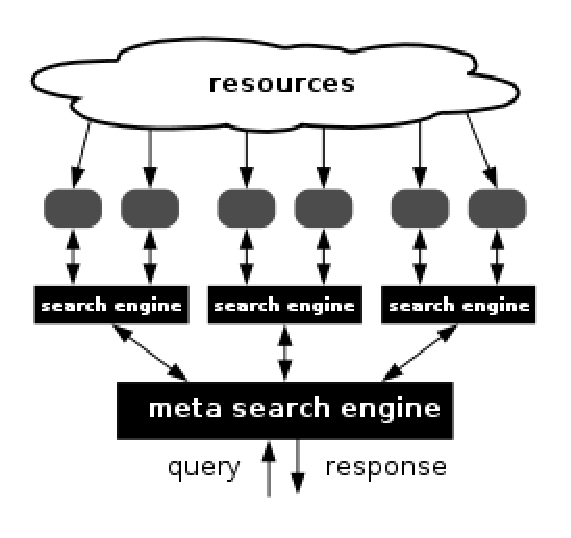
\includegraphics[width=0.5\textwidth,height=5cm]{figures/MetaSE.eps}
%  \caption{元搜索引擎工作流程草图}\label{fig:metase}
%\end{figure}
%
%国外元搜的发展比国内更成熟,无论界面设计,还是搜索技术都有大量可借鉴之处,这里简单介绍几个比较典型的元搜及其基本功能。
%\section{Savvy Search}
%睿智搜索(Savvy Search)是世界上第一个元搜索引擎,由科罗拉多州立大学研究生Daniel Dreilinger开发,1995年3月正式上线。
%睿智搜索运行在五台机器上,三个Sun SpackStation,两个IBM RS 6000s,其设计关注于平衡最大化精度、最小化计算及网络资源消耗两个相互冲突的目标,根据对各个独立搜索引擎长期的观察,确使每次提交给睿智搜索的检索词,依据系统历史统计数据,向最可能返回相关结果的独立搜索引擎提交检索请求,不仅确保精度,还减少了向所有独立搜索引擎提交查询的开销。
%睿智搜索是一个并行检索的元搜索引擎,可调用二十一个独立搜索引擎,检索包括WEB、USENET新闻组、软件、参考工具、人、技术报告等信息。每次最多可同时检索五个搜索引擎的数据库,也可以作为独立的搜索引擎使用。它还支持布尔查询,由于并非所有成员搜索引擎都能正确处理布尔操作符,搜索结果可能并不精确。它还允许用户指定每个搜索引擎返回结果的数目,如选择“聚合结果”选项,系统将对结果集作去重处理。默认情况下,它只显示各个独立搜索引擎前二十条命中记录。另外,它还支持包括中文在内的二十三种语言版本的搜索功能。
%1999年10月14日,CNet网络集团宣布以2200万美元股票和现金组合的形式将其收购,此时睿智搜索已经融合了三百多个网络搜索引擎的搜索结果,月均使用用户达到百万。
%
%\section{Meta Crawler}
%1994年,华盛顿大学研究生Eric Selberg和助理教授Oren Etzioni共同开发出Meta Crawler,并在1995年7月发布。Meta Crawler与Savvy搜索同年开发同年发布,人们常误以为它是世界上第一个元搜索引擎。1995年初,Meta Crawler已经运行在四个AlphaStation工作站上,日均处理几万条查询,给华盛顿大学宽带造成巨大的压力。1995 年夏,两人成立NetBot公司进行商业推广,但是由于没有明确的盈利模式,还需要向独立搜索引擎支付查询费用,不得己将使用权转让给Go2Net。2000年,Go2Net与InfoSpace 合并,虽然Meta Crawler仍提供独立的元搜索服务,地位已是今非昔比。
%Meta Crawler聚合了Google,Yahoo!,Bing,Ask.com,About.com,MIVA,LookSmart和其他主流搜索引擎的结果,提供网页、图片、视频、新闻的搜索服务。在高级搜索页面,用户可以设置最大等待时长(5秒至2分钟)和每个搜索引擎返回结果的最大数目(10、20、30),对各个独立搜索引擎的结果集成,删除重复的URL和死链接,将排序结果以统一的形式显示给用户。
%
%根据Eric Selberg自己的介绍,他们仅仅使用3到5个月的时间开发完成Meta Crawler,其中最复杂的一块就是网络处理,网络协议、并行I/O上占用了绝大部分时间。在开发时两人完全没有考虑过具体的商业模式,只是在发布后才逐渐摸索出一套商业模式:通过在搜索结果中显示独立搜索引擎的推广广告,实现利润共享。Eric认为,元搜面对的问题有很多,主要包括三点:(1)资源发现,能够自动发现新的搜索引擎并将其加入到独立搜索引擎列表;(2)用户认同,把用户的注意力从独立搜索引擎吸引到元搜;(3)商业模式,很难找到一个让所有独立搜索引擎提供商都满意的商业模式。
%
%\section{Dogpile}
%1996年,Aaron Flin创立了Dogpile,11月正式投入运营。1999年8月,以价值5500万美元的股票和现金作价卖给Go2Net,使得Go2Net旗下同时拥有了两个最受欢迎的元搜索引擎:Meta Crawler与Dogpile。2000年8月,InfoSpace与Go2Net集团合并,但Meta Crawler和Dogpile继续分开运营。2002年初,InfoSpace又以1,000万美元的低价收购Excite和Web Crawler,以麾下四个最著名的元搜索引擎独霸元搜索市场。
%
%Dogpile聚合了顶级搜索引擎Google、Yahoo!、Bing、Ask.com和About.com的搜索结果,并在2005年4月、2005年7月、2007年4月同匹兹堡大学(Pittsburgh University)、宾夕法尼亚大学(Pennsylvania State University)、昆士兰科技大学(Queensland University of Technology)研究人员合作,使用上万个查询词,估计几个顶级搜索引擎搜索结果的重复率情况。研究发现,主要搜索引擎(包括Google,Yahoo!,Ask,Bing)搜索结果的重复率低于4\%,2007年的研究结果甚至低于1\%,从而以此证明任何单个独立搜索引擎都不能完全满足用户的检索需求,元搜的存在是有价值的,它可以弥补独立搜索引擎覆盖率不足的问题,聚合多个独立搜索引擎的搜索结果,给用户更多相关的结果。
%
%\section{Excite}
%1994年,斯坦福大学(Stanford University)的Graham Spencer,Joe Kraus,Mark Van Haren,Ryan McIntyre,Ben Lutch和Martin Reinfried共同创立了Excite,提供包括门户、搜索引擎、电子邮箱、即时信息等多种在线服务。1994年7月,国际数据集团(International Data Group)向其投资10万美元用于开发一个在线服务网站,并于1995 年12月正式上线。1996 年1月,George Bell(错失过以75万美元收购Google的良机)以CEO的身份加盟Excite,并主持收购两个搜索引擎Magellan和WebCrawler。
%1996年4月4日,Excite首发200万股股票。由于经营不善,1998年3月31日其净损失竟达到近3千万美元,1999年1月19日@Home Network公司以67亿美元的价格将其收购,并组建新公司Excite@Home,融合@Home的高速网络服务和Excite搜索及门户网站,专注于提供个性化的网络内容服务。由于接二连三的商业决策失误,2001年9月13日Excite@Home申请破产保护,期间Iwon.com与InfoSpace联合投中Excite域名和品牌。2001年12月16日,Iwon.com启用新的Excite门户,并更名为Excite网络公司,继续经营Excite、iWon和另一个门户MyWay。InfoSpace则拥有和运营Excite的网络搜索部分。
%2004年3月Ask Jeeves(如今的Ask.com)将Excite网络公司收购,并在2005年,与InfoSpace就美国区Excite业务达成和解,双方共同承担市场成本、共享Excite 搜索业务的利润。
%
%\section{Web Crawler}
%1994年4月20日,由华盛顿大学(Washington Uiversity)学生Brian Pinkerton开发的Web Crawler发布上线,成为世界上第一个提供全文搜索的网络搜索引擎。1995 年6月1 日,美国在线将其收购,又在1997年4月1日转手卖给Excite,2001年Excite@Home破产后又将其出售给InfoSpace。最初,Web Crawler拥有独立的抓取程序和网页数据库,其主要收入来源于搜索结果页面投放的广告费,在并入InfoSpace以后,作为元搜索引擎向用户提供搜索服务。
%
%\section{Vivisimo}
%
%
%\section{Ixquick}
%Ixquick是David Bodnick于1998年研发并推出的一个元搜索引擎,自称是全球最大中介搜索引擎,目前支持14个搜索引擎的搜索结果。2000年,Ixquick被一家荷兰公司Surfboard Holding B.V收购。Ixquick背后的独立搜索引擎包括:Teoma,EntireWeb,All the Web,Ask,Bing,Cuil,Exalead,Gigablast,Lycos,AltaVista,WiseNut,LookSmart,Netscape,Open Directory, Qkport, Wikipedia,Statesman,Yahoo与Blekko,不含Google。
%
%2006年6月27日,Ixquick声明删除用户详细浏览信息,并保证在48小时内清除提交搜索的用户IP地址和其他个人信息。2009年1月28日宣布完全停止对用户IP地址的记录。
%截止2010年1月,Ixquick已经处理了12亿次查询请求。根据Ixquick公司背景介绍,它是世界上隐私保护做得最好的搜索引擎公司,从2006年起,开始专注对用户隐私的保护,做到不记录用户IP地址、cookies,不搜集而且不与第三方分享用户个人数据,提供安全的、加密的HTTPS/SSL连接。
%
%Ixquick直言提供相似搜索服务的搜索引擎,包括Google、Yahoo!和Bing,以及元搜索市场上,拥有三家马车的InfoSpace是其主要竞争对手。它目前还未上市,在过去的5年里(2006年起)一直都是盈利的,资金充裕,其盈利模式并无特别之处,在搜索结果页面显示相关的“赞助结果”,按照点击次数向广告客户收取费用,但每页显示的“赞助结果”不超过3条,而且全部放到搜索结果的首尾两端。
%
%由于Ixquick难以记忆和拼写,该公司于2009年启用新的域名Startpage\footnote{See http://www.startpage.com/}。有消息称,Ixquick 正在开发邮件服务系统。
%\section{Mamma}
%1996年,由加拿大人Herman Tumurcuoglu开发的网站Mamma.com
%\footnote{\href{http://www.mamma.com/}{http://www.mamma.com/}}
%正式发布上线。2005年12月22日,Mamma.com以1590万美元收购一家搜索技术公司Copernic,并发行238万股股票。Mamma.com 能够有效整合多个顶级搜索引擎的搜索结果,赢得“搜索引擎之母”的称号。它支持常用检索语法在不同搜索引擎之间的转换,还提供通过Email订制搜索结果的特色服务。Mamma.com还是一个广告网络公司,通过在线推介创收。
%
%\section{Kartoo}
%2002年04月25日,Laurent Baleydier和Nicholas Baleydier两兄弟联合开发的Kartoo\footnote{See http://www.kartoo.com/}上线,它是一个可视化元搜索引擎,以图形界面的形式展示搜索结果,通过关键词建立语义连接,将搜索结果生成一个聚类图,方便用户选择、缩小搜索范围。2010年1月,由于不明原因关闭。
%
%Kartoo使用的可视化技术是Laurent团队研究三年的成果,使用球形结点代替搜索结果条目,并通过球形节点的大小反映页面的重要程度。Kartoo最引人注目的地方在结点间的语义连接,如果搜索条目之间存在连接,则使用语义关键词标示节点之间的连线。Kartoo易于使用,并且富有趣味性,代价就是加载过慢。
%
%与国际市场形成鲜明对比,国内元搜市场鲜见成功的案例。我们下面介绍国内几个昙花一现的元搜:

%\subsection{比比猫}
%2005年1月1日,新加坡人朱明谦(Kim Choo)和李昌日联合创立了比比猫(Bbmao),并在2006年02月发布上线,它是中国第一家聚类元搜索引擎,通过聚类技术和个人网络收藏夹改善搜索结果。
%
%朱明谦对中国市场的分析可以归纳为以下几点:(1)中国搜索引擎市场差异化程度比较低,元搜的机会比较大。传统搜索引擎公司在底层搜索技术投入巨大,Bbmao 则更注重以上层的数据处理技术、智能搜索技术求生存。(2)大多数元搜没有核心技术,仅仅是整合其他搜索引擎的结果。只要有核心技术,公司就一定有价值,而Bbmao的核心技术就是聚类技术。(3)与独立搜索引擎合作共赢,独立搜索引擎提供搜索结果和竞价排名广告,元搜借着竞价排名广告收入分成。在06年,Bbmao的首席财务执行官Bill Milewski透露,Bbmao的盈利主要靠广告,并协议和Google等各大搜索引擎对广告利润分成。Bbmao期望成为一个社会化搜索引擎网站,其根本是发挥Web 2.0的内核——个人应用,靠用户改善搜索结果,就像Google通过搜索结果的点击改善排名。其特点可以归结为以下几点:
%\begin{itemize}
%  \item 资源聚合:同时提供Google,百度,雅虎,搜狗和爱问五大搜索引擎组合搜索或单个搜索结果,搜索结果排名是根据网页在各个搜索引擎中结果中出现的次数及排名来确定的,并明确标示各条结果在相应搜索引擎中的排名信息;
%  \item 聚类:在搜索结果页面左侧,呈现聚类列表,由用户点击选择目标类别,优化查询结果;
%  \item 去重:采用公司开发的FeatureMatch技术;
%  \item 快照:提供搜索结果预览;
%  \item 网络搜藏夹:注册用户享有的服务,方便用户收藏和共享,期望借此跟踪用户习惯,更好地为用户提供聚类结果,打造社会化搜索圈。
%  \item RenqiScore:使用人气得分技术向用户推荐高品质的相关会员,建立属于用户自己的交际网,还可以通过邀请朋友扩大交际圈。
%\end{itemize}
%
%2005年,Myspace创始人Brad Greenspan完成对Bbmao的注资,成为BroadWebAsia(BWA)集团在中国的第一笔投资。2006年3月,Bbmao的流量达到每天2万至3万,8月份超过7 万。Bbmao创建以后赢得的诸多赞誉,它启动“比比猫公益搜索”平台,以期打造互联网企业社会责任新方向。目前,Bbmao已经倒闭。Bbmao倒闭的原因有(1)用户习惯:它无法扭转已经习惯使用百度和Google的用户习惯。(2)它只是进行了非经营性网站的备案,并未获得经营性网站信息许可证,不能从事盈利性商业活动。(3)盈利模式单一:它主要与合作伙伴间的点击付费分成。
%
%\subsection{万纬}
%由上海万纬信息技术有限公司在1999年12月推出,是中国第一个元搜索引擎,集成了包括Google,Yahoo!,HotBot,AltaVista等8个英文搜索引擎,中文雅虎,搜狐、新浪、中文Excite、中文Google等12个中文搜索引擎,起正式版本2002年发布,功能比较完善。
%
%万纬搜索提供的高级搜索功能包括:(1)允许布尔查询,支持AND/OR;(2)结果排列方式有四种选择,包括相关度、时间、网站分类、引擎;(3)选择最大等待结果的时间,7秒到1分钟,默认20秒。(4)允许设置显示的查询结果个数,10到200个,默认为20个。遗憾地是,万纬在2007年7月份就已经停止查询服务。
%
%\subsection{搜乐}
%搜乐是广州明智科技有限公司推出的一个元搜索引擎。目前,搜乐整合了Google、百度、必应、搜狗、有道、搜搜和中搜等搜索引擎的搜索信息,并支持自动去重。
%主页功能显示,搜乐支持对网页、图片、视频、文档、新闻和微博的搜索,其中文档搜索包含的格式有Doc、XLS、PPT、PDF、RTF和TXT。
%
%在“设置”中可由用户指定(1)界面语言,包括中文繁体和简体。(2)搜索语言可不限。(3)每页显示结果3到100条。(4)是否在结果页中显示“推广”项;(5)是否允许在结果页中显示“赞助链接”。
%
%高级选项模仿了部分Google高级搜索的设置,添加对关键词出现位置的设定,包括文档的任何地方、仅标题、仅正文、仅URL和指向文档的链接。此外,它还支持对单个网站的搜索。目前搜乐不支持任何搜索,只有图片和视频展示页面。根据58同城招聘信息,明智科技正在招聘.NET软件工程师(2012年4月11日)和网站美工(2012 年3月21 日),组建创业团队。该公司主营产品是蓝月亮VOD点播系统。
%
%\subsection{名捕}
%名捕根据搜索类别,提供不同的资源列表方便用户选择,见下表:
%\begin{table}[htbp]
%\centering
%\begin{tabular}{|c|c|}
%    \hline\hline
%    搜索类别 & 资源网站列表\\
%    \hline
%    网页 & 百度、搜搜、搜狗、有道、中搜、必应、雅虎、谷歌、即刻\\
%    图片 & 雅虎、新浪、必应、搜狗\\
%    音乐 & 新浪、搜狗、雅虎、狗狗、搜搜\\
%    视频 & 新浪、土豆、优酷、搜搜、搜狗、谷歌、乐视\\
%    软件 & 天空、Enet、华军、百度、ZOL、Pchome、新浪\\
%    新闻 & 谷歌、有道、搜搜、必应、百度、搜狗\\
%    知识 & 知道、雅虎、百科、搜搜、搜狗\\
%    博客 & 搜搜、百度、有道、爱问、奇虎、搜狗、谷歌\\
%    论坛 & 谷歌、中搜、奇虎、贴吧、搜搜\\
%    词典 & 搜搜、爱词霸、海词、有道、沪江、词酷\\
%    财经 & 和讯、金融界、谷歌、搜牛、中金\\
%    购物 & 谷歌、有道、淘宝、当当、卓越\\
%  \hline
%\end{tabular}
%\end{table}
%
%它只提供搜索引擎的切换,不提供结果排名聚合。从根本上来讲,它只提供了针对各个搜索类别比较权威的站点,供用户挑选。此外,名捕还在首页提供了几个不错的资源——搜索大全、儿歌大全、晨曦五笔、绝妙好词。
%
%\subsection{P搜}
%P搜是刘洪照历经四年研发的成果,它聚合了百度、Google、Yahoo!、搜狗、有道、搜搜和必应的搜索结果,经过去重,重排,缩小搜索范围,精确查找信息。
%根据其本人介绍,第一版搜鸿元搜索引擎(sohong.cn)由于技术瓶颈问题,一直没突破速度限制,搜索耗时略长。在2009年4月份他重写搜鸿,突破了技术瓶颈,并陆续添加竞价排名和后台管理模块,并易名为新牛元搜索(ccniu.com)。后受到115聚合搜索的影响,历时一周对新牛改写,实现了各个模块的松耦合,并通过API整合各个模块,
%
%2009年9月升级到第二版。2010年初新牛上线,放弃服务端处理模式,改用Ajax模式,速度比以前要慢,但节省服务器开支,由于没有独立服务器,Ajax版本超过两秒,原服务端处理在1秒以内。至2011年2月,历经5次代码重写,多次更新,新牛算法趋于合理,搜索结果排序更加人性化。2011年5月8日改版并易名为P搜,采用镜像psou.cn。
%
%\subsection{马虎聚搜}
%马虎聚搜是BroadWebAsia(BWA)集团在中国投资的第一家互联网公司,提供基于搜索引擎的多种互联网服务。马虎聚搜声称经过技术测试,国内通用搜索引擎在搜索结果前两页当中,重复率约占5-16\%。该公司拥有独特的FeatureMatch技术,可以大幅减少搜索结果中的重复信息。(FeatureMatch——Bbmao)
%
%搜索发现,基本上和百度的搜索结果一样,不同之处在于马虎聚搜会过滤掉百度文库、百度翻译、能够提供直接下载的搜索结果条目,并在每个搜索结果条目前加注序号。如切换到独立搜索引擎,会自动弹出对应的搜索引擎搜索结果页面,若切换到Google、Bing,还会出现中文乱码。支持收藏和预览功能,但最多返回10页搜索结果。对音乐、图片、视频的搜索直接跳转到百度的搜索页面。
%
%\subsection{佐意}
%佐意网的前身是一佐网络,始建于1998年3月,2007年3月正式更名为佐意网,并启用新域名。佐意是一个集成搜索引擎,提供网页,新闻,软件,游戏,动画,音乐,影视,地图等信息的搜索,能够自动屏蔽掉色情木马不良网站,减少用户的烦恼。2010年10月11日,佐意网终止搜索服务,转为一个以BLOG为主,并提供相关查询的综合性网站。2011年7月1日,佐意官网宣布停止运营,终止所有服务。
%
%\subsection{Juxit}
%Juxit是Reuben Boyd 于2004年创建和发布的,声称是第一个聚合了中英双语的元搜索引擎。它聚合了Google中文,Yahoo中文,百度,搜狗,MSN,Wisenut 和 Looksmart 的搜索结果。Juxit包含购物、旅行、新闻、图片、视频和音频搜索,并提供预览功能。它支持免费的、按点击次数收费的广告,并推出联盟计划(affiliate program),向广告客户支付转介佣金。此外,它还允许广告穿插到搜索结果中。目前,Juxit已经停止运营。
%
%目前中国国内还出现过很多其他元搜,我们将它们全部收录于表~\ref{tbl:cnmetase}。
%\begin{table}[htbp]
%\centering
%\caption{中国元搜索引擎目录}\label{tbl:cnmetase}
%\begin{tabular}{|l|l|l|l|l|}
%    \hline\hline
%    名称 & 介绍 & 发布时间 & 状态\\
%    \hline
%    \href{http://www.bioon.com/multisearch.htm/}{生物谷} &  张发宝开发,搜索时同时展开多个页面 & 2001年10月 & 正常\\
%    \hline
%    \href{http://www.suotianxia.com}{索天下} &  -- & 2006年12月14日 & 关闭\\
%    \hline
%        &  华南师范大学附属中学的叶古于2003年开发,采用CooRank & & \\
%    \href{http://coo.hsfz.net/fish/}{MetaFisher} & 自动分网页评级系统优化排序,CooWord2Beta关键词 & 2003年 & 关闭\\
%        & 析归纳算法增加搜索深度和广度,CooSimil滤重 & & \\
%     \hline
%        & 提供了Google+百度,Google+Yahoo!,Google+Yahoo! & & \\
%    \href{http://www.xisoso.com/}{Xisoso} &  三种组合的搜索结果,搜索结果还提供del.icio.us  & -- & 关闭 \\
%        & 标签和天天网摘(365Key),还支持自动聚类功能 & & \\
%    \hline
%    \href{http://www.baidugoo.com/}{Baidugoo} &  -- & -- & 关闭\\
%    \hline
%    \href{http://www.bydou.com/}{北斗搜索} &  深入搜索、相关搜索、可评价结果 & -- & 关闭 \\
%    \hline
%    \href{http://www.ejear.com/}{壹家搜} &  聚合百度、Google中文、Yahoo!中文的搜索 & & \\
%        & 结果,据称对相似结果的处理有其特色 & 2005年11月 & 正常\\
%    \hline
%    \href{http://www.bbmao.com/}{比比猫} &  聚类、在线收藏共享 & -- & 关闭\\
%    \hline
%    \href{http://www.hensou.com/}{狠搜} &  -- & -- & 关闭\\
%    \hline
%    \href{http://www.kwindsoft.com/k-metasearch/}{K风元搜索} &  聚合、收藏功能 & 2007年01月02日 & 关闭\\
%    \hline
%    \href{http://cn.xooda.com/}{Xooda中国} &  支持16个国家和地区的搜索,而中文支持Google、&&\\
%        & 百度、中文雅虎、爱问、搜狗等10多个搜索引擎 & 2007年02月16日 & 关闭\\
%    \hline
%    \href{http://www.seekle.cn/}{Seekle} &  聚合百度、Google、搜狗、Yahoo!的搜索结果 & 2007年12月30日 & 关闭\\
%    \hline
%    \href{http://www.pifa.us/}{PIFA} &  -- & 2008年01月13日 & 关闭\\
%    \hline
%    \href{http://www.sohong.cn/}{搜鸿元搜索} &  艺鸿开发,后易名为搜牛、P搜,支持去重、 &&\\
%        & 重排、预览、收藏等功能,使用方便快捷 & 2008年02月19日 & 正常\\
%    \hline
%        & 基于Ajax技术,聚合谷歌、百度、雅虎、&&\\
%    \href{http://www.metasoo.cn/}{觅搜} & 一搜、搜狗、有道等搜索引擎搜索结果 & -- & 正常\\
%        & 允许用户自行设置各搜索引擎权重 & & \\
%    \hline
%    \href{http://www.deyeb.com/}{Deyeb} &  董一萌开发的社会化元搜 & -- & 关闭\\
%    \hline
%    \href{http://www.soseen.com/}{搜星} &  聚合百度、搜狐、新浪、Google等搜索引擎,可搜索精选网址 & -- & 关闭\\
%    \hline
%    \href{http://www.1qiso.com/}{一起搜} &  自称全球最大中文元搜,聚合12个中外搜索引擎结果 & -- & 关闭\\
%    \hline
%    \href{http://www.jopee.cn/}{Jopee} &  聚合百度、Google、搜狗、必应、有道、Ask,简单切换 & -- & 正常\\
%    \hline
%        & 聚合百度、Google、搜狗、雅虎和中搜,提供网页、 & &\\
%    \href{http://www.someta.com/}{搜魅} & 资讯、图片、网站查询,宣称是最优秀的中文元搜索 & 2009年 & 正常\\
%        & “搜魅聚合”等于是百度搜索 & & \\
%%    \hline
%%    \href{http://www.mangken.com/}{芒肯} &  -- & -- & 关闭\\
%%    \hline
%%    \href{http://www.souk.cn/}{搜客} &  -- & -- & 关闭\\
%%    \hline
%%    \href{http://www.yok.com/}{YOK} &  -- & -- & 关闭\\
%%    \hline
%%    \href{http://www.souk.cn/}{搜客} &  -- & -- & 关闭\\
%%    \hline
%%    \href{http://www.koooi.com/}{酷爱} &  -- & -- & 关闭\\
%  \hline
%\end{tabular}
%\end{table}
%
%\subsection{市场层面}
%从用户使用的习惯来看,中国大多用户已经习惯使用单个搜索引擎比如百度、Google,查询所需信息。目前,由于Google退出中国市场,将服务器移到香港,但时断时续的状态导致用户分流,这就部分造就了如今百度一家独大的局面。
%
%根据iResearc的统计数据,2012年2月Google全球搜索引擎市场份额从1月份的75.9\%下降到72.1\%,同时Yahoo!的市场份额则从11.1\%上升到16.5\%。即便真如Google前CEO Eric Smith所言,称Google实际市场份额是包含了一部分垂直搜索引擎市场的份额的,但Google行业龙头老大的地位短时期内是无法撼动的。
%
%从易观国际在2011年第四季度的数据可以看到,百度在中国搜索引擎市场上的份额达到78.3\%,而处于第二位的Google则只有16.7\%,搜狗、搜搜等其他搜索引擎的市场份额之和只有5\%。这种格局同iResearch全球搜索引擎市场格局颇为相似,即一家独大,在中国,百度处于绝对垄断地位。相对PC机搜索市场而言,中国无线搜索市场分布则比较均匀,但百度的份额仍然是最大的一块。
%
%iResearch在2011年底预计中国搜索引擎市场规模到2013年将达到438亿元人民币,而根据易观国际在2010年的预测,到2013年市场规模将达到313亿元人民币,虽然二者相差将近100亿,但从整体趋势来看,搜索市场增长的潜力是巨大。
%
%在这个巨头环立的市场中,元搜要想生存、获得一席之地,首先要有有明确的用户群和市场定位,推崇用户体验至上;其次,由于元搜会分走独立搜索引擎的部分流量,影响其广告业务,应努力寻找同独立搜索引擎合作的结合点,尽可能营造计较有利的发展环境,打消独立搜索引擎对元搜的戒心,避免成为众矢之的。如2008年4 月7日,李彦宏到上海交大演讲。在互动时有学生提到使用“百Google度”同时搜索百度和Google,李彦宏称“元搜索没有生命力”,然而给出的理由却很牵强,“元搜索可以同时查询多个搜索引擎的站点,但用户不需要那么复杂的结果,而且相当多的人习惯了用百度”,并奉劝创业者不要往视频搜索上“撞”。
%
%\subsection{技术层面(智能选择、去重、聚类、推荐、重排)}
%市场再大,没有核心技术的互联网公司终究无法在这个市场立足,元搜更需要核心技术的支撑。通过分析,国内元搜基本可以归为两种模式:
%\begin{itemize}
%  \item 框架调用:为用户提供在不同搜索引擎之间进行快速切换,基本无核心技术,容易复制;实际上也不能归为元搜的范畴,没有什么参考价值。
%  \item 聚合调用(直接抓取或API调用)——用户一次提交,系统把多个独立搜索引擎搜索结果,经过滤重、重排等处理,返回更为合理的聚合结果。其中,虑重、重排等技术是核心,难以复制。
%\end{itemize}
%第2种模式被普遍认可,它主要存在以下几个问题:
%\begin{itemize}
%  \item 比使用单个独立搜索引擎查询所需时间更长
%  \item 处理高级检索时,需要将检索语句转换为不同独立搜索引擎的标准格式,转换效果不佳并影响到搜索的效率
%  \item 搜索结果依赖于独立搜索引擎数据库的大小、数据的质量
%  \item 只能从独立搜索引擎数据库中获取搜索结果的有限信息,如排名、摘要信息等,影响搜索结果排名的可信性
%  \item 由于部分独立搜索引擎的盈利模式的特殊性,导致其搜索结果中出现竞价排名的商业广告,智能识别出其中的“赞助广告”是一个不小的挑战。识别出不相关的结果页面,如包含木马病毒、色情信息的网页或网站对于改善用户体验是十分重要的,而实现这一目标难度不小
%  \item 由于不同搜索引擎对搜索结果的显示格式也是不同的,以一种统一的方式聚合异构的搜索结果展示给用户,处理起来比较复杂,也是影响搜索效率的又一个障碍
%  \item 元搜经常需要批量访问独立搜索引擎的数据库,但由于各主流搜索引擎对访问都设置了上限,信息的查全率会受到很大影响
%  \item 随着访问量的增加,服务器端流量、数据处理的压力明显增加,因此硬件要求颇高
%\end{itemize}
%元搜是为弥补传统搜索引擎的不足而出现的一种辅助搜索工具。因此,必须从数据库选择、查询分派、文本选择、虑重、结果聚合、排名和显示等环节寻求突破,而且这些也是未来元搜研究的重点。
%
%\subsection{法律层面}
%由于元搜没有独立的数据库,需要在用户提交查询以后,选择并抓取独立搜索引擎的数据库。显然,元搜受制于人,可能会由于频繁抓取独立搜索引擎的数据库,影响独立搜索引擎正常服务,或增加其服务成本而面临诉讼风险。这是否又是一桩“只需州官放火,不许百姓点灯”的经典案例呢?具体的互联网数据信息的访问是否受限,可查询相关法规。
%
%\subsection{国内环境的特殊性}
%在中国搜索市场上,曾经出现过很多元搜索引擎,有些还很优秀,比如Bbmao、万纬,但后来由于不明原因陆续倒闭。其他类型的元搜多是单人开发,核心技术几乎为零,从界面设计到服务性能都与国外成熟的元搜相差甚远,甚至还有一些打着元搜的旗号,使用小偷程序,安装恶意软件,给用户留下很差的印象。因此,若要在中国推出元搜,让更多用户了解元搜的角色和价值、依赖单个搜索引擎的局限性、遗漏重要信息的代价、重拾用户对元搜的信心是首先要做的工作。
%
%另一方面,由于国内对知识产权保护不力,产品一经推出会即刻产生一批跟风者,这种良莠不齐的混乱状况,会给产品形象带来很大的冲击。因此,产品一定要有特色,并有明确的目标受众,能够明显区别于其他类似产品。由于国内众多企业道德问题饱受公众质疑,因此一个坚决抵制不良信息,努力呈现高品质内容,尽力追求企业良知的搜索引擎公司一定是大众所渴望的,也一定可以走得更远。
%
%\subsection{商业模式}
%在早期,搜索引擎多作为技术提供商,通过为其他网站提供搜索服务收取服务费。2001年,互联网泡沫破灭后,多转向竞价排名的方式。现在主流搜索引擎商业模式(Google的AdWords、百度的竞价排名)由是Bill Gross提出的,“在搜索结果页面显示广告,根据用户点击向广告客户收费”。该模式有两个特点:一是点击付费(Pay Per Click,简称PPC),用户不点击则广告客户不用付费;二是竞价排名,根据广告客户的付费多少给结果排名。
%
%2003年6月,Google推出一种免费的广告计划AdSense,它是一种面向站长的广告服务。网站发布者为访客提供Google网页和网站搜索功能,借由在搜索结果页面投放Google 广告以获取收益。目前,各大搜索引擎已经开始使用这种模式。
%
%元搜依赖独立搜索引擎而存在,从搜索业务的角度来看,元搜与独立搜索引擎是竞争关系。由于市场份额多被少数独立搜索引擎瓜分殆尽,元搜要在这种不对等的关系中生存和发展,必须提出一种既不会伤及独立搜索引擎利益,又能够持续提供搜索业务的方案,即与独立搜索引擎合作。元搜同独立搜索引擎该如何合作,国外元搜市场比较成功的商业模式,比如InfoSpace 公司可以为我们提供一些借鉴。
%
%InfoSpace公司通过旗下的三个元搜索引擎——Dogpile, WebCrawler, MetaCrawler向用户提供搜索服务,是一个上市公司,因此需要按规定定期发布公司相关信息。
%2012年3月9日,InfoSpace发布报告,在Business小节中披露,Google, Yahoo!, Bing和其他搜索引擎被InfoSpace称作内容提供商(Content Providers),并且如果部分内容提供商,如Google,Yahoo!向其支付内容发布的费用,则称它们为搜索客户(Search Customer)。
%
%在Search Revenue Source一节中有记录,其主要收入来自内容提供商向其搜索服务中投放的付费广告。广告客户根据用户点击向独立搜索引擎支付费用,InfoSpace 则从中提成。报告中还披露,在2010年和2011年,Google和Yahoo!两家公司占其全部收入来源95\%以上,而其中Google占绝大部分。报告坦言,如若这两家公司减少面向InfoSpace 的业务,或者对之前协议的价格产生异议的话,必然会对InfoSpace的业务和财务构成造成巨大冲击。

%\chapter{Academic Search Engine}
%\chapter{Shopping Search Engine}

